\documentclass[11pt]{article}
\usepackage[utf8]{inputenc}
\usepackage[T1]{fontenc}
\usepackage[spanish,es-noquoting,es-tabla]{babel}
\usepackage[a4paper,margin=2.5cm]{geometry}
\usepackage{amsmath}
\usepackage{amssymb}
\usepackage{amsthm}
\usepackage{graphicx}
\usepackage{booktabs}
\usepackage{longtable}
\usepackage{float}
\usepackage{multirow}
\usepackage{array}
\usepackage{algorithm}
\usepackage{algpseudocode}
\usepackage[font=small,labelfont=bf]{caption}
\usepackage[colorlinks=true,linkcolor=black,citecolor=blue,urlcolor=blue]{hyperref}
\usepackage[section]{placeins}
\renewcommand{\topfraction}{0.9}
\renewcommand{\bottomfraction}{0.8}
\renewcommand{\textfraction}{0.07}
\renewcommand{\floatpagefraction}{0.75}
\setcounter{topnumber}{3}
\setcounter{bottomnumber}{2}
\setcounter{totalnumber}{5}
\usepackage{setspace}
\onehalfspacing
\decimalpoint
\floatname{algorithm}{Algoritmo}
\algrenewcommand\algorithmicrequire{\textbf{Entrada:}}
\algrenewcommand\algorithmicensure{\textbf{Salida:}}

\newtheorem{proposicion}{Proposición}

\begin{document}

% ============================================================
% PORTADA
% ============================================================
\begin{center}

\includegraphics[height=1.6cm]{logo_uninorte.jpg}

\vspace{1.8em}

{\LARGE\textbf{Pronóstico de la tasa de desempleo en Colombia}}\\[4pt]
{\LARGE\textbf{mediante agregación local entrópica de expertos}}

\vspace{2em}

\textbf{Santiago Hurtado} \hspace{2.5em} \textbf{Juan Marín} \hspace{2.5em} \textbf{Andrés Parejo}

\vspace{4pt}

Universidad del Norte --- Ciencia de Datos

\vspace{1em}

Noviembre de 2026
\end{center}

\vspace{2em}

% ============================================================
% RESUMEN
% ============================================================
\begin{abstract}
\noindent
Entre los modelos de aprendizaje automático evaluados en un trabajo previo sobre el desempleo colombiano, el de menor error cambiaba según la volatilidad reciente del mercado laboral. A partir de esa observación, este trabajo propone ALEE (agregación local entrópica de expertos), una combinación de tres pronosticadores programados explícitamente ---persistencia, regresión de Nadaraya-Watson del cambio y cambio estacional medio--- cuyos pesos se localizan según el estado del mercado laboral, se restringen al símplex y se regularizan con divergencia de Kullback-Leibler hacia una combinación global, con más fuerza cuando la evidencia local es escasa. El problema es convexo, tiene solución única y se resuelve por descenso de espejo con descenso monótono. ALEE se compara con los ocho modelos de regresión del curso (KNN, Ridge, Lasso, regresión bayesiana, árbol de decisión, Random Forest, XGBoost y SVR) y con LightGBM, mediante validación anidada de origen móvil, en la tasa de desempleo de Colombia (2002--2025) y en ocho países adicionales. ALEE tiene el menor error en los nueve conjuntos y en las cinco métricas evaluadas, con reducciones del RMSE de 21\,\% a 33\,\% frente al mejor modelo del curso, y supera a los nueve modelos de comparación de forma significativa en cada conjunto (Diebold-Mariano-HLN y Giacomini-White con corrección de Holm, $p<0.05$ en las 81 comparaciones) y entre conjuntos (Wilcoxon con Holm, $p=0.035$ frente a cada modelo). La ablación muestra que la combinación aprendida supera al promedio simple en siete de los nueve conjuntos, pero que la localización por estado solo aporta de forma significativa en dos.
\end{abstract}

\noindent\textbf{Palabras clave:} desempleo; mercado laboral; combinación de pronósticos; aprendizaje automático; series de tiempo; Colombia.

\newpage

% ============================================================
% 1. INTRODUCCIÓN
% ============================================================
\section{Introducción}
\label{sec:intro}

El desempleo es uno de los indicadores más vigilados del desempeño macroeconómico de un país, pues sintetiza tanto la capacidad de la economía para generar empleo como la presión que ejerce la población en edad de trabajar sobre el mercado laboral \cite{phillips1958,okun1962}. Su comportamiento ha sido objeto de estudio recurrente debido a su volatilidad estructural y a fenómenos asociados como la informalidad laboral, particularmente en economías en desarrollo \cite{sanchez2013,berrio2019}. En Colombia, el Departamento Administrativo Nacional de Estadística (DANE) produce mensualmente estos indicadores a través de la Gran Encuesta Integrada de Hogares \cite{dane_geih}, y el Banco de la República los distribuye en su portal de series estadísticas históricas \cite{banrep2025series}.

El episodio más disruptivo de las últimas dos décadas en esta serie fue la pandemia de COVID-19: el Banco de la República documentó un deterioro histórico del mercado laboral colombiano en 2020, con una destrucción de empleo sin precedentes en zonas urbanas y rurales \cite{banrep2020covid}. Este tipo de choques plantea un reto particular para cualquier modelo de pronóstico y, como se muestra más adelante, es también el episodio en el que el desempeño de los modelos resulta menos estable.

Tradicionalmente, el desempleo se ha analizado con la econometría clásica de series de tiempo \cite{boxjenkins1976}, evaluando propiedades como la estacionariedad mediante pruebas de raíz unitaria \cite{dickeyfuller1979}. En los últimos años se le han aplicado modelos de aprendizaje automático, incluidas redes profundas \cite{madaras2024}, aunque las comparaciones a gran escala muestran que, en series univariadas, los modelos genéricos de aprendizaje automático no siempre superan a métodos que incorporan explícitamente la estructura temporal \cite{makridakis2018,makridakis2020}. En un trabajo previo de este proyecto se diagnosticó, para las seis series mensuales del mercado laboral colombiano \cite{banrep_sf_mercado}, una multicolinealidad severa entre las versiones de área metropolitana y nacional de cada indicador \cite{hair2019}, y se evaluaron siete modelos de aprendizaje automático ---entre ellos Ridge \cite{hoerl1970}, Lasso \cite{tibshirani1996}, Random Forest y XGBoost--- con validación anidada. Ninguno se distinguió estadísticamente de los demás en el conjunto de confianza de modelos \cite{hansen2011}, y el de menor error variaba según la volatilidad reciente: los árboles ganaban con volatilidad baja, los modelos lineales con volatilidad media y la persistencia con volatilidad alta. Una regla de combinación de pesos fijos \cite{timmermann2006} no puede aprovechar ese cambio.

La combinación de pronósticos con pesos que varían en el tiempo o con el punto que se pronostica tiene antecedentes. \cite{li2001} estima los pesos con una regresión de núcleo, \cite{chenmaung2023} los hace variar en el tiempo con un estimador lineal local y los aplica al desempleo de Estados Unidos, y los ensambles dinámicos arbitrados \cite{cerqueira2017} los adaptan con un meta-modelo que predice el error de cada experto. Para series macroeconómicas, \cite{elliotttimmermann2005} muestra que condicionar los pesos a un régimen mejora el pronóstico, aunque su régimen es discreto y latente. Los \textit{local prediction pools} \cite{oelrich2024} condicionan los pesos de una combinación de densidades a la precisión local de cada experto y los encogen hacia pesos iguales cuando hay pocos datos, y \cite{dang2027} combina en línea con descenso de espejo entrópico dentro de celdas discretas de contexto. Para Colombia, el antecedente más cercano usa procesos gaussianos con reducción de dimensionalidad interpretable \cite{perezrosero2025}, sin combinar expertos.

La revisión anterior deja tres limitaciones concretas. En primer lugar, los combinadores que condicionan los pesos lo hacen al tiempo, a regímenes discretos o a la precisión de densidades, y ninguno localiza de forma continua sobre el estado observado del mercado laboral los pesos de un pronóstico puntual. En segundo lugar, cuando hay pocos meses parecidos al actual, como en el choque de 2020, los pesos estimados localmente se vuelven inestables, y los métodos que los encogen lo hacen hacia pesos iguales y con una fuerza fija, no hacia la combinación global ni en proporción a la evidencia local disponible. En tercer lugar, los modelos genéricos de aprendizaje automático deben aprender la estacionalidad y la persistencia de la serie a partir de pocas observaciones, mientras que expertos sencillos las incorporan de forma directa.

Para cubrir esas limitaciones, este trabajo propone ALEE (agregación local entrópica de expertos), que combina tres expertos programados explícitamente ---persistencia, regresión de Nadaraya-Watson del cambio y cambio estacional medio--- con pesos que se localizan con un núcleo sobre el estado del mercado laboral, se restringen al símplex y se regularizan con divergencia de Kullback-Leibler hacia la combinación global, con una fuerza inversamente proporcional al tamaño efectivo de la muestra local. El problema de los pesos es convexo, tiene solución única y se resuelve por descenso de espejo con descenso monótono. ALEE se evalúa en la tasa de desempleo de Colombia y en ocho países más, con validación anidada de origen móvil, las mismas variables para todos los competidores y pruebas de significancia con corrección por comparaciones múltiples. Supera de forma significativa a los ocho modelos de regresión del curso y a LightGBM en los nueve conjuntos, con reducciones del RMSE de 21\,\% a 33\,\% frente al mejor de ellos, y la ablación muestra que la ventaja se debe sobre todo a los expertos y solo en parte a la localización por estado.

La pregunta de investigación es si una combinación de expertos con pesos locales por estado pronostica la tasa de desempleo a un mes mejor que los modelos de regresión vistos en el curso; la hipótesis es que ALEE tiene menor error cuadrático que cada uno de ellos.

El resto de este artículo está organizado de la siguiente manera: la Sección~\ref{sec:metodos} describe los datos y la metodología propuesta; la Sección~\ref{sec:diseno} presenta el diseño experimental y los modelos de referencia; la Sección~\ref{sec:resultados} expone los resultados, la validación estadística y su discusión; finalmente, la Sección~\ref{sec:conclusiones} presenta las conclusiones y el trabajo futuro.

\newpage

% ============================================================
% 2. DATOS Y METODOLOGÍA
% ============================================================
\section{Datos y metodología}
\label{sec:metodos}

\subsection{Formulación del problema}

Sea $y_t$ la tasa de desempleo nacional en el mes $t$ y $\mathbf{x}_t\in\mathcal{X}=\mathbb{R}^p$ un vector de variables construido únicamente con información disponible al cierre del mes $t$. El problema es el pronóstico a un mes: aprender $f:\mathcal{X}\to\mathcal{Y}=\mathbb{R}$ tal que $\hat y_{t+1}=f(\mathbf{x}_t)$, sin usar nunca información del mes $t+1$. La pérdida de referencia es el error cuadrático medio,
\[
\mathcal{L}_{\mathrm{MSE}}=\frac{1}{n}\sum_{t=1}^{n}\left(y_{t+1}-\hat y_{t+1}\right)^2 .
\]
En lo que sigue, $K$ es el número de expertos de ALEE, $f_k$ el pronóstico del experto $k$, $e_{s,k}$ su error fuera de muestra en el mes pasado $s$, $z(\mathbf{x})$ el estado del mercado laboral, $w\in\Delta_K$ los pesos de la combinación en el símplex de dimensión $K$, y $h$, $\tau$ y $\lambda$ los tres hiperparámetros del modelo.

\subsection{Datos y análisis exploratorio}
\label{sec:datos}

\textbf{Problema principal (Colombia).} Los datos provienen del DANE (Gran Encuesta Integrada de Hogares) y los distribuye el Banco de la República \cite{dane_geih,banrep2025series}: tasa global de participación, tasa de desempleo y tasa de ocupación, nacionales y de las 13 áreas metropolitanas, mensuales, de enero de 2001 a diciembre de 2025, sin valores faltantes. La ocupación y la participación nacionales se excluyen como predictoras por la identidad contable $TD = 1 - TO/TGP$.

La Figura~\ref{fig:eda} reúne los cuatro patrones del análisis exploratorio que condicionan el diseño del modelo. La serie es persistente y sufrió un choque extremo en 2020 (panel a), de modo que un experto de persistencia es una referencia natural y los meses del choque tienen pocos antecedentes parecidos. El cambio mensual tiene un patrón estacional marcado y estable, con un salto medio de unos 3 puntos en enero (panel b): un experto que sume al último dato el cambio típico del mes incorpora esa estructura de forma directa. La autocorrelación del nivel decae lentamente, mientras que la del cambio mensual se concentra en los rezagos 12 y 24 (panel c). Por último, entre los modelos del trabajo previo el de menor error cambia con la volatilidad reciente (panel d): XGBoost con volatilidad baja, Ridge con volatilidad media y SVR con volatilidad alta, lo que motiva pesos que dependan del estado del mercado laboral.

\begin{figure}[H]
\centering
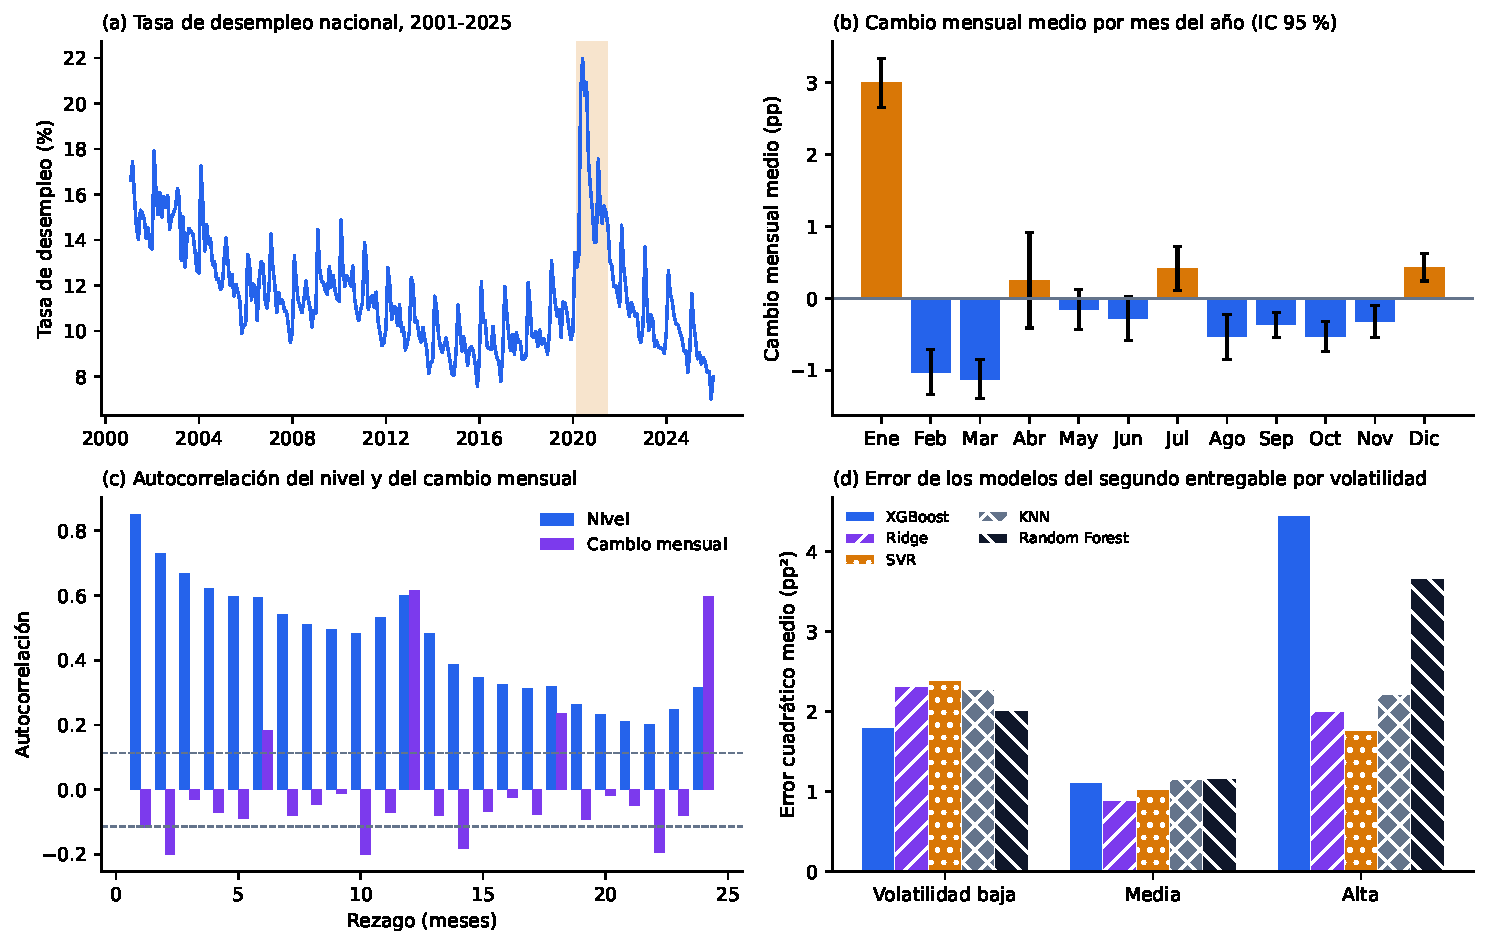
\includegraphics[width=\linewidth]{figuras/fig_eda.pdf}
\caption{Patrones del análisis exploratorio. (a) Tasa de desempleo nacional, con el choque de 2020 en ámbar. (b) Cambio mensual medio por mes del año, con su intervalo de confianza del 95\,\%. (c) Autocorrelación del nivel y del cambio mensual; las líneas discontinuas son las bandas de $\pm1.96/\sqrt{n}$. (d) Error cuadrático medio fuera de muestra de cinco modelos del trabajo previo por tercil de la volatilidad de los últimos tres meses.}
\label{fig:eda}
\end{figure}

\textbf{Conjuntos adicionales.} Para probar la generalización se usan ocho tasas de desempleo mensuales sin desestacionalizar, todas elegidas antes de ver resultados sobre ellas. Tres se definieron con el protocolo original: Estados Unidos \cite{fred_unratensa}, España \cite{eurostat_une} y México (ENE/ENOE de INEGI, distribuida por la OCDE) \cite{oecd_lfs}. Las otras cinco provienen de la misma base de la OCDE \cite{oecd_lfs} (población de 15 años o más, sin ajuste estacional) y se eligieron con criterios fijados de antemano ---serie mensual, al menos 240 meses consecutivos y que no sea un promedio móvil de tres meses---: Canadá, Australia, Japón, Alemania y Corea del Sur. Como no existen indicadores de área para estos países, se construyen las mismas variables sin ellas (14 variables). Octubre de 2025 no se publicó en Estados Unidos por el cierre del gobierno federal y se rellenó por interpolación lineal; ninguna otra serie tiene valores faltantes.

\textbf{Licencia.} Todos los datos son públicos. Los del DANE y el Banco de la República son información pública de libre acceso; la serie de FRED proviene de la Oficina de Estadísticas Laborales de Estados Unidos y es de dominio público; Eurostat y la OCDE permiten reutilizar sus datos citando la fuente (licencia CC BY 4.0).

\textbf{Variable objetivo.} La Tabla~\ref{tab:objetivo} resume la distribución de la tasa de desempleo en cada conjunto. Los niveles van de 0.9\,\% (Japón) a 27.1\,\% (España), y la distribución es asimétrica a la derecha en todos los casos, sobre todo en Corea del Sur y Colombia, por los episodios de desempleo alto. Como valores atípicos se cuentan los cambios mensuales fuera de las vallas externas de Tukey (más de tres rangos intercuartílicos). Los más importantes son los choques de 2020 (Colombia, Estados Unidos, México y Canadá), la crisis asiática de 1998 en Corea y la de 2009 en España; los de Japón y Canadá en las décadas de 1950 y 1960 reflejan la estacionalidad más marcada de esos años. Los atípicos no se eliminan ni se recortan, porque son justamente los episodios que un modelo de pronóstico debe enfrentar.

\begin{table}[H]
\centering
\caption{Distribución de la tasa de desempleo (\%) en cada conjunto: periodo, número de meses, media, desviación estándar, mínimo, máximo, asimetría y número de cambios mensuales atípicos (fuera de $[Q_1-3\,\mathrm{RIC},\,Q_3+3\,\mathrm{RIC}]$).}
\label{tab:objetivo}
\small
\resizebox{\textwidth}{!}{\begin{tabular}{lcccccccc}
\toprule
Conjunto & Periodo & Meses & Media & Desv. & Mín. & Máx. & Asimetría & Cambios atípicos \\
\midrule
Colombia & 2001--2025 & 300 & 11.61 & 2.45 & 7.02 & 21.97 & 1.09 & 2 \\
EE.UU. & 1948--2026 & 946 & 5.65 & 1.74 & 2.40 & 14.40 & 0.84 & 5 \\
España & 1986--2026 & 486 & 16.09 & 4.77 & 7.80 & 27.10 & 0.20 & 1 \\
México & 2000--2026 & 321 & 3.80 & 0.95 & 2.15 & 6.43 & 0.44 & 1 \\
Canadá & 1955--2026 & 862 & 7.23 & 2.20 & 1.90 & 14.30 & 0.30 & 14 \\
Australia & 1978--2026 & 584 & 6.49 & 1.87 & 3.25 & 12.13 & 0.70 & 1 \\
Japón & 1955--2026 & 861 & 2.73 & 1.20 & 0.90 & 5.80 & 0.60 & 9 \\
Alemania & 1991--2026 & 429 & 6.47 & 2.57 & 2.80 & 12.20 & 0.14 & 0 \\
Corea del Sur & 1989--2026 & 453 & 3.40 & 1.10 & 1.80 & 8.80 & 1.87 & 5 \\
\bottomrule
\end{tabular}}
\end{table}

\subsection{Ingeniería de características}
\label{sec:variables}

Con $y_t$ la tasa nacional y $\mathbf{x}_t$ la información del mes $t$, se construyen
\begin{equation}
\begin{gathered}
\ell_{t,k}=y_{t-k+1},\quad k\in\{1,2,3,6,12\};\\
\bar y_{t,m}=\frac{1}{m}\sum_{j=0}^{m-1}y_{t-j},\qquad s_{t,m}=\Big(\frac{1}{m-1}\sum_{j=0}^{m-1}(y_{t-j}-\bar y_{t,m})^2\Big)^{1/2},\quad m\in\{3,6,12\},
\end{gathered}
\label{eq:variables}
\end{equation}
más el mes codificado como $(\sin(2\pi\,\mathrm{mes}_t/12),\cos(2\pi\,\mathrm{mes}_t/12))$, un índice de tendencia y, en Colombia, los tres indicadores de las 13 áreas metropolitanas del mes $t$. Son 17 variables en Colombia y 14 en los demás conjuntos. Todas usan solo meses $\le t$, de modo que $\hat y_{t+1}=f(\mathbf{x}_t)$ nunca ve el valor que pronostica. En Colombia quedan 288 observaciones, con objetivos de enero de 2002 a diciembre de 2025. No hay variables categóricas. El estado del mercado laboral que usa ALEE para localizar es $z(\mathbf{x}_t)=(s_{t,3},\,y_t-\bar y_{t,12})$, estandarizado: la volatilidad reciente y la brecha del último dato frente a su media anual.

\textbf{Escalamiento y fuga de información.} Todas las variables se construyen solo con información pasada respecto al mes pronosticado. Los modelos que lo requieren (KNN, Ridge, Lasso, regresión bayesiana y SVR) estandarizan las variables con la media y la desviación del tramo de entrenamiento de cada pliegue, y aplican esa misma transformación a la validación y a la prueba; ALEE estandariza internamente con el mismo criterio. Ningún ajuste de preprocesamiento usa datos del pliegue evaluado, para evitar la fuga de información hacia el futuro \cite{kapoor2023}. Las particiones respetan el orden temporal (Sección~\ref{sec:entrenamiento}).

\subsection{Modelo propuesto: ALEE}
\label{sec:modelo}

\textbf{Idea central.} ALEE pronostica con una combinación convexa de tres expertos sencillos, y elige los pesos de esa combinación en cada mes según qué tan bien le fue a cada experto en los meses pasados parecidos al actual. Cuando hay pocos meses parecidos, los pesos se acercan a una combinación global estable. La Figura~\ref{fig:diagrama} resume el modelo y el Algoritmo~\ref{alg:alee} lo describe paso a paso.

\begin{figure}[H]
\centering
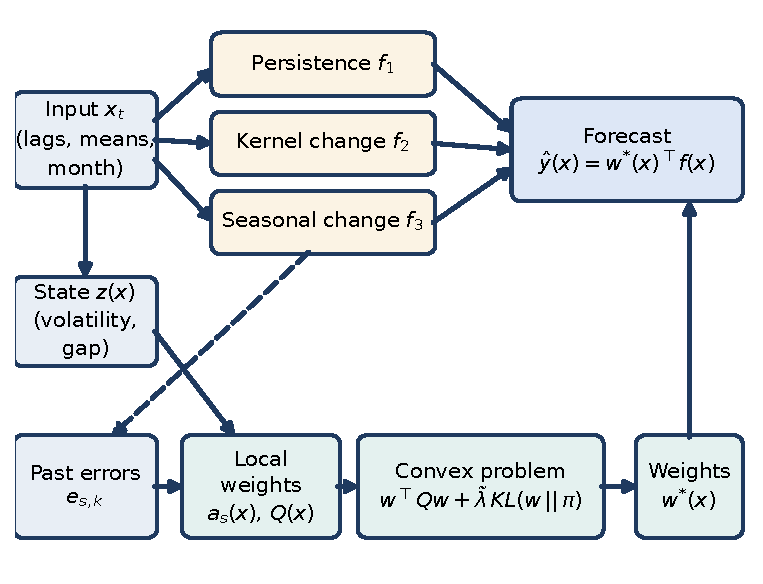
\includegraphics[width=\linewidth]{figuras/fig_diagrama_alee.pdf}
\caption{Diagrama de ALEE. Arriba, los tres expertos pronostican a partir de la entrada y el pronóstico final los combina. Abajo, cómo se obtienen los pesos: los errores pasados de los expertos se ponderan según la similitud de estado con el mes actual, y los pesos resuelven un problema convexo regularizado hacia la combinación global. La flecha discontinua indica que los errores pasados se registran fuera de muestra, en ventana expansiva.}
\label{fig:diagrama}
\end{figure}

\textbf{Expertos.} ALEE combina $K=3$ expertos programados en NumPy, cada uno entrenado solo con información anterior al punto que pronostica: (i) persistencia, $f_1=y_t$, que funciona bien cuando la serie cambia de nivel bruscamente; (ii) núcleo-cambio, $f_2=y_t$ más una regresión de Nadaraya-Watson \cite{nadaraya1964,watson1964} del cambio mensual sobre las variables estandarizadas, que capta relaciones no lineales con el pasado reciente; y (iii) estacional, $f_3=y_t$ más el cambio medio histórico del mismo mes del año, encogido hacia cero, que capta el patrón estacional.

\textbf{Pesos locales.} Para un punto $\mathbf{x}$ con estado $z(\mathbf{x})$ ---volatilidad de los últimos 3 meses y brecha entre $y_t$ y su media de 12 meses, estandarizadas--- los meses pasados reciben pesos de localización
\begin{equation}
a_s(\mathbf{x}) \propto \exp\!\left(-\frac{\lVert z(\mathbf{x})-z_s\rVert^2}{2h^2}\right)\gamma^{\,n-1-s}, \qquad \gamma = 0.5^{1/\tau},
\label{eq:local}
\end{equation}
con ancho de banda $h$ y vida media $\tau$. El núcleo da más peso a los meses con un estado parecido, y el decaimiento, a los más recientes. Con ellos se forma la matriz de errores locales $Q(\mathbf{x})=\sum_s a_s(\mathbf{x})\, e_s e_s^\top$, semidefinida positiva, de modo que $w^\top Q(\mathbf{x}) w$ es el error cuadrático local de la combinación $w$.

\textbf{Combinación.} Los pesos resuelven
\begin{equation}
w^*(\mathbf{x}) = \arg\min_{w\in\Delta_K}\; g(w) := w^\top Q(\mathbf{x})\,w + \tilde\lambda(\mathbf{x})\,\mathrm{KL}(w\,\Vert\,\pi),
\qquad \tilde\lambda(\mathbf{x}) = \lambda\,\frac{\operatorname{tr} Q(\mathbf{x})}{K}\,\frac{n_{\mathrm{ref}}}{n_{\mathrm{eff}}(a)},
\label{eq:alee}
\end{equation}
donde $\pi$ son los pesos globales (la misma combinación sin localización, en el interior del símplex), $n_{\mathrm{eff}}(a) = 1/\sum_s a_s^2$ es el tamaño efectivo de la muestra local \cite{kish1965} y $n_{\mathrm{ref}}$ el de los pesos con solo decaimiento temporal. El término de Kullback-Leibler evita que los pesos se sobreajusten a pocos meses: cuando hay pocos meses parecidos al actual ---como en el choque de 2020---, $\tilde\lambda$ crece y la combinación se acerca a $\pi$. El pronóstico es $\hat y = \sum_k w_k^* f_k(\mathbf{x})$. El problema se resuelve con descenso de espejo proximal (gradiente exponenciado \cite{kivinen1997}) con paso $\eta=1/L$, $L = 2\max_{ij}|Q_{ij}|$, hasta que el cambio de los pesos en norma $\ell_1$ es menor que $10^{-10}$ o se cumplen 500 iteraciones.

\begin{algorithm}[H]
\caption{ALEE: entrenamiento y pronóstico de un mes}
\label{alg:alee}
\begin{algorithmic}[1]
\Require Datos $\{(\mathbf{x}_s,y_s)\}_{s=0}^{n-1}$ en orden temporal; hiperparámetros $h,\tau,\lambda$; punto nuevo $\mathbf{x}$
\Ensure Pronóstico $\hat y$
\For{$s=m_0,\dots,n-1$} \Comment{historial de errores en ventana expansiva}
  \State Ajustar los expertos $f_k^{(s)}$ solo con las filas $0,\dots,s-1$
  \State $e_{s,k}\gets y_s-f_k^{(s)}(\mathbf{x}_s)$ para $k=1,\dots,K$
\EndFor
\State $\pi\gets$ solución de \eqref{eq:alee} con $a_s\propto\gamma^{\,n-1-s}$ y previo uniforme \Comment{pesos globales}
\State Ajustar los expertos finales $f_k$ con las $n$ filas
\State Calcular $a_s(\mathbf{x})$ con \eqref{eq:local}, $Q\gets\sum_s a_s e_s e_s^\top$ y $\tilde\lambda$
\State $w\gets\pi$; $\eta\gets 1/(2\max_{ij}|Q_{ij}|)$
\Repeat \Comment{descenso de espejo proximal}
  \State $w\gets \left(w\odot e^{-2\eta Qw}\right)^{1/(1+\eta\tilde\lambda)}\odot\pi^{\eta\tilde\lambda/(1+\eta\tilde\lambda)}$, normalizado a $\sum_k w_k=1$
\Until{$\lVert w_{\text{nuevo}}-w\rVert_1<10^{-10}$ o 500 iteraciones}
\State \Return $\hat y=\sum_k w_k f_k(\mathbf{x})$
\end{algorithmic}
\end{algorithm}

\textbf{Propiedades.} Las tres propiedades siguientes no son resultados nuevos de optimización: se derivan de resultados conocidos y se verifican numéricamente en las pruebas unitarias del código.

\begin{proposicion}[Existencia y unicidad]
Si $\tilde\lambda>0$, el problema \eqref{eq:alee} tiene una única solución, y esta pertenece al interior de $\Delta_K$.
\end{proposicion}
\begin{proof}[Esbozo]
$w^\top Q w$ es convexa porque $Q\succeq0$, y $\mathrm{KL}(\cdot\Vert\pi)$ es estrictamente convexa y continua en $\Delta_K$ (con $0\log0=0$); su suma es estrictamente convexa y continua en un conjunto compacto y convexo, así que el mínimo existe y es único. Como la derivada de $w_k\log w_k$ tiende a $-\infty$ cuando $w_k\to0$, ningún punto de la frontera puede ser óptimo.
\end{proof}

\begin{proposicion}[Descenso monótono]
Con paso $\eta = 1/L$, $L=2\max_{ij}|Q_{ij}|$, la iteración del Algoritmo~\ref{alg:alee} no aumenta $g$ en ningún paso.
\end{proposicion}
\begin{proof}[Esbozo]
Sea $f(w)=w^\top Qw$. Para $u,w\in\Delta_K$, $f(u)-f(w)-\langle\nabla f(w),u-w\rangle=(u-w)^\top Q(u-w)\le\max_{ij}|Q_{ij}|\,\lVert u-w\rVert_1^2\le L\,\mathrm{KL}(u\Vert w)$, donde la última desigualdad es la de Pinsker. Luego $f$ es $L$-suave relativa a la entropía negativa, y el paso proximal con el término $\tilde\lambda\,\mathrm{KL}(\cdot\Vert\pi)$ tiene la forma cerrada del algoritmo; el lema de descenso de \cite{bauschke2017} garantiza entonces que $g(w_{t+1})\le g(w_t)$.
\end{proof}

\begin{proposicion}[Error acotado]
Para cualquier $\mathbf{x}$ y cualquier valor observado $y$, $|y-\hat y|\le\max_k|y-f_k(\mathbf{x})|$ y $(y-\hat y)^2\le\sum_k w^*_k\,(y-f_k(\mathbf{x}))^2$.
\end{proposicion}
\begin{proof}[Esbozo]
$\hat y$ es una combinación convexa de los $f_k(\mathbf{x})$; la primera desigualdad es la desigualdad triangular y la segunda, la de Jensen aplicada a la función convexa $u\mapsto u^2$.
\end{proof}

Además, con $\lambda\to\infty$ se recuperan los pesos globales $\pi$, y sin localización los pesos no dependen de $\mathbf{x}$.

\textbf{Qué es nuevo.} La localización por núcleo ya aparece en \cite{li2001}, los pesos condicionados a covariables que se encogen con poca información local en \cite{oelrich2024} y el descenso de espejo entrópico por contexto en \cite{dang2027}. ALEE reúne esas ideas en un mismo mecanismo para pronósticos puntuales: localiza de forma continua sobre un estado observado (no sobre el tiempo ni sobre celdas o regímenes discretos), regulariza hacia la combinación global y no hacia pesos iguales, ajusta la fuerza de esa regularización al tamaño efectivo de la muestra local y obtiene los pesos de un problema convexo con solución única. Una búsqueda en Scopus con cinco cadenas pre-registradas, cuatro complementarias y \textit{snowballing} hacia adelante (90 registros) no encontró un trabajo que reúna esas cuatro piezas.

\textbf{Implementación y complejidad.} El modelo, los expertos y el solucionador están implementados en NumPy, sin modelos de librería, en una clase compatible con \texttt{scikit-learn}. ALEE tiene tres hiperparámetros y no tiene parámetros entrenables por gradiente: lo que aprende es el historial de errores, de tamaño $(n-m_0)\times K$. La Tabla~\ref{tab:complejidad} resume el costo de cada etapa.

\begin{table}[H]
\centering
\caption{Complejidad asintótica de ALEE en tiempo y memoria, con $n$ meses, $p$ variables, $K$ expertos e $I$ iteraciones del descenso de espejo.}
\label{tab:complejidad}
\small
\begin{tabular}{p{7.6cm}ll}
\toprule
Etapa & Tiempo & Memoria \\
\midrule
Ajuste de los expertos con $s$ meses (ancho de banda por la mediana) & $O(s^2p)$ & $O(s^2)$ \\
Historial de errores en ventana expansiva ($s=m_0,\dots,n-1$) & $O(n^3p)$ & $O(n^2+nK)$ \\
Pesos globales $\pi$ & $O(nK^2+IK^2)$ & $O(K^2)$ \\
Pronóstico de un mes: localización, $Q(\mathbf{x})$ y descenso de espejo & $O(np+nK^2+IK^2)$ & $O(n+K^2)$ \\
\bottomrule
\end{tabular}
\end{table}

\begin{proposicion}[Complejidad]
Con $K$ e $I$ acotados, entrenar ALEE cuesta $O(n^3p)$ en tiempo y $O(n^2)$ en memoria, y pronosticar un mes cuesta $O(np)$, lineal en el tamaño del historial.
\end{proposicion}
\begin{proof}[Justificación]
Para cada $s=m_0,\dots,n-1$ el experto de núcleo calcula las $s^2$ distancias entre los meses anteriores en $O(s^2p)$ para fijar su ancho de banda, y $\sum_{s\le n}s^2p=O(n^3p)$; los otros dos expertos cuestan $O(s)$. Al pronosticar, las distancias del estado nuevo a los $n$ meses cuestan $O(np)$, la matriz $Q$ cuesta $O(nK^2)$ y cada iteración del descenso de espejo cuesta $O(K^2)$.
\end{proof}

% ============================================================
% 3. DISEÑO EXPERIMENTAL
% ============================================================
\section{Diseño experimental y modelos de referencia}
\label{sec:diseno}

\subsection{Particiones y validación cruzada anidada}
\label{sec:entrenamiento}

Los hiperparámetros de todos los modelos ---en ALEE, $h\in[0.05,3]$, $\tau\in[6,120]$ meses y $\lambda\in[10^{-3},100]$, en escala logarítmica--- se ajustan con optimización bayesiana (estimador de Parzen en árbol, 40 evaluaciones, 10 de arranque aleatorio) \cite{snoek2012,akiba2019} dentro de una validación anidada de origen móvil \cite{cerqueira2020}: \texttt{TimeSeriesSplit} con 5 pliegues externos y 3 internos y un \textit{gap} de un mes. Cada pliegue externo entrena con todos los meses anteriores a su tramo de prueba, y el pliegue externo nunca interviene en la elección de hiperparámetros. El bucle interno elige los hiperparámetros; el externo estima el desempeño del procedimiento completo, y de él provienen la media y la desviación estándar que se reportan. Los cinco pliegues externos suman 240 meses de prueba en Colombia, 775 en Estados Unidos, 395 en España, 255 en México, 705 en Canadá, 475 en Australia, 705 en Japón, 345 en Alemania y 365 en Corea del Sur.

El orden de las operaciones es lo que garantiza que no haya fuga de información \cite{kapoor2023}. Primero se fijan, solo con las fechas, las particiones externas e internas. Solo después, y dentro de cada pliegue, se estiman con las filas de su entrenamiento las medias y desviaciones de estandarización, el historial de errores de los expertos de ALEE y los hiperparámetros; las filas de evaluación se transforman con esos parámetros sin intervenir en su cálculo. La semilla es 42; la variabilidad se mide además con las semillas 43 a 51 (Sección~\ref{sec:ablacion}). Los experimentos se corrieron en un procesador AMD de 12 núcleos con Windows 11 y Python 3.13, con NumPy 2.5 \cite{harris2020}, pandas 3.1 \cite{mckinney2010}, SciPy 1.18 \cite{virtanen2020}, scikit-learn 1.9 \cite{pedregosa2011}, statsmodels 0.15 \cite{seabold2010}, Optuna 5.0 \cite{akiba2019}, XGBoost 3.4 \cite{chen2016}, LightGBM 4.7 \cite{ke2017}, scikit-posthocs 0.17 \cite{terpilowski2019} y Matplotlib 3.11 \cite{hunter2007}.

\subsection{Modelos de referencia}
\label{sec:baselines}

ALEE se compara con los ocho modelos de regresión del curso: KNN, Ridge \cite{hoerl1970}, Lasso \cite{tibshirani1996}, regresión bayesiana (\texttt{BayesianRidge}), árbol de decisión, Random Forest, XGBoost \cite{chen2016} y SVR con kernel RBF. Se agrega LightGBM \cite{ke2017} como método reciente de alto rendimiento. Todos usan las mismas particiones, el mismo preprocesamiento y el mismo presupuesto de ajuste.

\subsection{Métricas y pruebas de hipótesis}
\label{sec:protocolo}

\textbf{Métricas.} La métrica primaria es el RMSE medio de los cinco pliegues externos. Las secundarias son MAE, MAPE, $R^2$ y MASE, este último escalado por el error absoluto medio del ingenuo estacional dentro del entrenamiento de cada pliegue \cite{hyndman2006}. Se reportan media y desviación estándar entre pliegues.

\textbf{Pruebas por conjunto de datos.} ALEE se contrasta con cada uno de los $m=9$ modelos de comparación mediante la combinación mínima que exige el pronóstico de series de tiempo: (1) Diebold-Mariano con la corrección de Harvey-Leybourne-Newbold \cite{dieboldmariano1995,harveyetal1997}, sobre las mismas observaciones de prueba; (2) Giacomini-White condicional \cite{giacominiwhite2006}, con la diferencia de pérdida rezagada como instrumento (estadístico de Wald, $\chi^2$ con dos grados de libertad); y (3) la $t$ bayesiana correlacionada con región de equivalencia práctica (ROPE) \cite{coranibenavoli2015,benavoli2017}, sobre la diferencia relativa de RMSE por pliegue, con ROPE de $\pm1$\,\% y correlación igual a la proporción media de prueba; por la dependencia temporal, esta última se interpreta con cautela. Los valores $p$ se ajustan con Holm \cite{holm1979} por separado en cada prueba y en cada conjunto, con $\alpha=0.05$. Como tamaño de efecto se reportan la diferencia media de pérdida cuadrática con intervalo de confianza del 95\,\% por \textit{bootstrap} estacionario (bloque medio de 12 meses) \cite{politisromano1994}, la $d$ de Cohen y la $A_{12}$ de Vargha-Delaney \cite{varghadelaney2000}. Como complemento se calcula el conjunto de confianza de modelos (MCS) \cite{hansen2011} con $\alpha=0.10$ y bloques de 12 meses.

\textbf{Pruebas entre conjuntos.} Con los nueve conjuntos como bloques independientes se aplica Friedman con la corrección de Iman-Davenport, el post-hoc de Conover con Holm frente a ALEE como modelo de control y el Wilcoxon de rangos con signo pareado con Holm \cite{demsar2006,garciaherrera2008}; además se dibuja el diagrama de diferencia crítica y se calcula el signed-rank bayesiano \cite{benavoli2014}.

\subsection{Diseño del estudio de ablación, sensibilidad y costo}
\label{sec:ablacion}

La ablación aísla cada componente de ALEE en los nueve conjuntos, con una variante por componente y todo lo demás constante. Cada variante se ajusta con el mismo protocolo, se evalúa con las cinco métricas y se contrasta con ALEE completo mediante Diebold-Mariano-HLN con Holm dentro de cada conjunto. Se contrastan cinco hipótesis:
\begin{itemize}\setlength\itemsep{0pt}
\item \textbf{H1} (combinación aprendida): ALEE es mejor que el promedio simple de sus tres expertos.
\item \textbf{H2} (localización): ALEE es mejor que la misma combinación sin localización, en la que todos los meses pasados pesan igual.
\item \textbf{H3} (regularización adaptativa): ALEE es mejor que la variante con $\lambda$ fijo, sin el factor $n_{\mathrm{ref}}/n_{\mathrm{eff}}$.
\item \textbf{H4} (previo global): ALEE es mejor que la variante que regulariza hacia el promedio uniforme.
\item \textbf{H5} (complementariedad): ALEE es mejor que cada uno de sus expertos por separado.
\end{itemize}
La sensibilidad se mide con la variación entre semillas del optimizador en los cuatro conjuntos originales (42 a 46 para ALEE, y 42 a 51 para Random Forest, XGBoost y LightGBM en Colombia), con un mapa del RMSE sobre una rejilla de $(h,\lambda)$ con $\tau=60$, y con una curva de aprendizaje en Estados Unidos: periodo de prueba fijo (los últimos 156 meses) y ventanas de entrenamiento de 60 a 777 meses, con los hiperparámetros de ALEE fijos en la mediana de los elegidos en los pliegues. El costo computacional se mide en el último pliegue de Colombia, con los hiperparámetros elegidos en ese pliegue y cada modelo en un proceso independiente.

\subsection{Pre-registro, iteraciones de diseño y desviaciones}
\label{sec:preregistro}

El protocolo (métricas, pruebas, $\alpha$ y conjuntos adicionales) se escribió y congeló el 5 de noviembre de 2026, antes de la validación confirmatoria. La versión pre-registrada de ALEE tenía cinco expertos; la versión de tres expertos que se presenta aquí resulta de una iteración de diseño posterior a esa validación, que quitó los dos expertos de ridge, ajustada con validación anidada y declarada como tal. La Tabla~\ref{tab:registro} separa lo pre-registrado de lo agregado después. En total se evaluaron diez iteraciones de diseño sobre los 240 meses de Colombia, todas registradas con fecha; por eso los ocho conjuntos adicionales, evaluados una sola vez con el modelo congelado, son la evidencia principal de generalización. Todas las tablas, pruebas y figuras de este documento se reproducen desde un único \textit{script} a partir de los datos públicos citados.

\begin{table}[H]
\centering
\caption{Qué se fijó antes de la validación confirmatoria y qué se agregó después.}
\label{tab:registro}
\scriptsize
\begin{tabular}{p{4.2cm}p{2.3cm}p{7.6cm}}
\toprule
Elemento & Estado & Motivo o detalle \\
\midrule
Métrica primaria, particiones, $\alpha$ & Pre-registrado & Protocolo congelado el 5 de noviembre de 2026. \\
Diebold-Mariano-HLN, Giacomini-White, MCS, Friedman & Pre-registrado & --- \\
Conjuntos adicionales (EE.UU., España, México) & Pre-registrado & Evaluados una sola vez, con el modelo congelado. \\
LightGBM & Pre-registrado & Método reciente fijado en el protocolo. \\
ALEE de tres expertos & Posterior & Iteración de diseño tras la validación confirmatoria: se quitaron los dos expertos de ridge. \\
Siete iteraciones de diseño más & Posterior & Otros expertos, otros estados de localización y otras reglas de combinación; ninguna se adoptó. \\
Cinco conjuntos más (Canadá, Australia, Japón, Alemania, Corea) & Posterior & Recomendados por la guía (al menos cinco conjuntos). Los países y sus criterios de inclusión se fijaron antes de descargarlos, y ALEE se evaluó una sola vez sobre ellos, congelado. \\
Regresión bayesiana y SVR solo RBF & Posterior & Exigidos por la guía del curso. \\
Prueba bayesiana con ROPE & Posterior & Exigida por la guía; ROPE de $\pm1$\,\% fijado antes de calcularla. \\
MAPE, $R^2$, MASE; Holm por prueba; Wilcoxon & Posterior & Exigidos por la guía. \\
Ablación con hipótesis, sensibilidad, costo & Posterior & Exigidos por la guía; ninguno modifica las predicciones de ALEE. \\
\bottomrule
\end{tabular}
\end{table}

\newpage

% ============================================================
% 4. RESULTADOS Y DISCUSIÓN
% ============================================================
\section{Resultados y discusión}
\label{sec:resultados}

\FloatBarrier
\subsection{Resumen del montaje experimental}

Se comparan diez modelos ---ALEE, los ocho modelos de regresión del curso y LightGBM--- en nueve conjuntos de datos: Colombia y ocho países adicionales, con entre 240 y 775 meses de prueba cada uno (4\,260 en total). Todos usan las mismas cinco particiones externas de origen móvil, el mismo preprocesamiento y 40 evaluaciones de optimización bayesiana con semilla 42. La métrica primaria es el RMSE medio de los pliegues externos, en puntos porcentuales (pp); las secundarias son MAE, MAPE, $R^2$ y MASE. Las pruebas por conjunto contrastan a ALEE con cada uno de los nueve modelos de comparación, con corrección de Holm por prueba y $\alpha=0.05$.

\FloatBarrier
\subsection{Desempeño predictivo global}

La Tabla~\ref{tab:rmse} resume la métrica primaria y la Tabla~\ref{tab:metricas} reporta las cinco métricas de los diez modelos en los nueve conjuntos. ALEE tiene el menor RMSE en los nueve conjuntos, y también el menor MAE, el menor MAPE, el mayor $R^2$ y el menor MASE en todos ellos. Frente al mejor modelo del curso en cada conjunto, el RMSE baja entre 21\,\% (Japón, 0.149 frente a 0.188 de la regresión bayesiana) y 33\,\% (Colombia, 0.817 frente a 1.219 de Ridge). Entre los modelos del curso no hay un ganador estable: el mejor es la regresión bayesiana en cuatro conjuntos, Lasso en tres, Ridge en uno y SVR en otro; los métodos de árboles, incluido LightGBM, quedan en general detrás de los lineales. El MASE de ALEE es menor que 1 en los nueve conjuntos (entre 0.13 y 0.55): su error es claramente menor que el del ingenuo estacional.

\begin{table}[H]
\centering
\caption{RMSE medio de los cinco pliegues externos (pp). En negrita el mejor modelo de cada conjunto y subrayado el segundo. $^{\dagger}$: ALEE es significativamente mejor que ese modelo (Diebold-Mariano-HLN, $p$ ajustado por Holm $<0.05$). Las desviaciones estándar están en la Tabla~\ref{tab:metricas}.}
\label{tab:rmse}
\small
\resizebox{\textwidth}{!}{\begin{tabular}{lccccccccc}
\toprule
Modelo & Colombia & EE.UU. & España & México & Canadá & Australia & Japón & Alemania & Corea del Sur \\
\midrule
ALEE & \textbf{0.817} & \textbf{0.380} & \textbf{0.280} & \textbf{0.281} & \textbf{0.437} & \textbf{0.240} & \textbf{0.149} & \textbf{0.226} & \textbf{0.325} \\
\midrule
KNN & 1.251$^{\dagger}$ & 0.820$^{\dagger}$ & 1.613$^{\dagger}$ & 0.533$^{\dagger}$ & 1.052$^{\dagger}$ & 0.656$^{\dagger}$ & 0.510$^{\dagger}$ & 0.816$^{\dagger}$ & 0.789$^{\dagger}$ \\
Ridge & \underline{1.219}$^{\dagger}$ & 0.555$^{\dagger}$ & 0.581$^{\dagger}$ & 0.386$^{\dagger}$ & 0.731$^{\dagger}$ & 0.468$^{\dagger}$ & 0.199$^{\dagger}$ & 0.345$^{\dagger}$ & 0.472$^{\dagger}$ \\
Lasso & 1.601$^{\dagger}$ & \underline{0.541}$^{\dagger}$ & \underline{0.369}$^{\dagger}$ & 0.373$^{\dagger}$ & \underline{0.601}$^{\dagger}$ & 0.359$^{\dagger}$ & 0.198$^{\dagger}$ & 0.298$^{\dagger}$ & 0.464$^{\dagger}$ \\
Regresión bayesiana & 1.289$^{\dagger}$ & 0.551$^{\dagger}$ & 0.556$^{\dagger}$ & 0.386$^{\dagger}$ & 0.631$^{\dagger}$ & \underline{0.342}$^{\dagger}$ & \underline{0.188}$^{\dagger}$ & \underline{0.288}$^{\dagger}$ & \underline{0.438}$^{\dagger}$ \\
Árbol de decisión & 1.475$^{\dagger}$ & 0.748$^{\dagger}$ & 3.333$^{\dagger}$ & 0.738$^{\dagger}$ & 1.090$^{\dagger}$ & 0.702$^{\dagger}$ & 0.616$^{\dagger}$ & 0.864$^{\dagger}$ & 0.728$^{\dagger}$ \\
Random Forest & 1.298$^{\dagger}$ & 0.737$^{\dagger}$ & 1.735$^{\dagger}$ & 0.524$^{\dagger}$ & 0.953$^{\dagger}$ & 0.686$^{\dagger}$ & 0.521$^{\dagger}$ & 0.852$^{\dagger}$ & 0.786$^{\dagger}$ \\
XGBoost & 1.284$^{\dagger}$ & 0.611$^{\dagger}$ & 1.569$^{\dagger}$ & 0.542$^{\dagger}$ & 0.862$^{\dagger}$ & 0.606$^{\dagger}$ & 0.562$^{\dagger}$ & 0.731$^{\dagger}$ & 0.805$^{\dagger}$ \\
SVR (RBF) & 1.283$^{\dagger}$ & 0.712$^{\dagger}$ & 0.820$^{\dagger}$ & \underline{0.369}$^{\dagger}$ & 0.730$^{\dagger}$ & 0.440$^{\dagger}$ & 0.337$^{\dagger}$ & 0.395$^{\dagger}$ & 0.503$^{\dagger}$ \\
LightGBM & 1.452$^{\dagger}$ & 0.720$^{\dagger}$ & 1.854$^{\dagger}$ & 0.549$^{\dagger}$ & 0.799$^{\dagger}$ & 0.647$^{\dagger}$ & 0.542$^{\dagger}$ & 0.858$^{\dagger}$ & 0.832$^{\dagger}$ \\
\bottomrule
\end{tabular}}
\end{table}

{\scriptsize\setlength{\tabcolsep}{3pt}
\begin{longtable}{llccccc}
\caption{Todas las métricas (media $\pm$ desviación estándar entre los cinco pliegues externos) de los nueve modelos en los nueve conjuntos. En negrita, el mejor valor de cada métrica en cada conjunto.}\label{tab:metricas}\\
\toprule
Conjunto & Modelo & RMSE & MAE & MAPE (\%) & $R^2$ & MASE \\
\midrule
\endfirsthead
\toprule
Conjunto & Modelo & RMSE & MAE & MAPE (\%) & $R^2$ & MASE \\
\midrule
\endhead
\bottomrule
\endfoot
Colombia & ALEE & \textbf{0.817 $\pm$ 0.328} & \textbf{0.586 $\pm$ 0.156} & \textbf{5.15 $\pm$ 0.71} & \textbf{0.660 $\pm$ 0.287} & \textbf{0.550 $\pm$ 0.209} \\
 & Ridge & 1.219 $\pm$ 0.638 & 0.906 $\pm$ 0.431 & 7.63 $\pm$ 2.66 & 0.195 $\pm$ 0.947 & 0.849 $\pm$ 0.475 \\
 & KNN & 1.251 $\pm$ 0.633 & 0.883 $\pm$ 0.314 & 7.61 $\pm$ 1.93 & 0.305 $\pm$ 0.425 & 0.848 $\pm$ 0.435 \\
 & SVR (RBF) & 1.283 $\pm$ 0.655 & 0.941 $\pm$ 0.433 & 7.88 $\pm$ 2.47 & 0.167 $\pm$ 0.849 & 0.897 $\pm$ 0.528 \\
 & XGBoost & 1.284 $\pm$ 1.004 & 0.888 $\pm$ 0.547 & 7.37 $\pm$ 2.87 & 0.418 $\pm$ 0.285 & 0.889 $\pm$ 0.745 \\
 & Regresión bayesiana & 1.289 $\pm$ 0.834 & 0.994 $\pm$ 0.635 & 8.28 $\pm$ 4.44 & -0.029 $\pm$ 1.534 & 0.929 $\pm$ 0.646 \\
 & Random Forest & 1.298 $\pm$ 0.826 & 0.911 $\pm$ 0.423 & 7.79 $\pm$ 2.31 & 0.374 $\pm$ 0.230 & 0.892 $\pm$ 0.598 \\
 & LightGBM & 1.452 $\pm$ 0.997 & 1.048 $\pm$ 0.540 & 8.95 $\pm$ 3.25 & 0.245 $\pm$ 0.291 & 1.023 $\pm$ 0.724 \\
 & Árbol de decisión & 1.475 $\pm$ 1.049 & 1.085 $\pm$ 0.611 & 8.98 $\pm$ 3.14 & 0.047 $\pm$ 0.859 & 1.062 $\pm$ 0.805 \\
 & Lasso & 1.601 $\pm$ 1.027 & 1.260 $\pm$ 0.810 & 10.70 $\pm$ 6.02 & -0.917 $\pm$ 3.189 & 1.150 $\pm$ 0.685 \\
\midrule
EE.UU. & ALEE & \textbf{0.380 $\pm$ 0.292} & \textbf{0.210 $\pm$ 0.054} & \textbf{3.65 $\pm$ 1.24} & \textbf{0.901 $\pm$ 0.123} & \textbf{0.220 $\pm$ 0.066} \\
 & Lasso & 0.541 $\pm$ 0.274 & 0.363 $\pm$ 0.088 & 6.56 $\pm$ 2.54 & 0.814 $\pm$ 0.150 & 0.376 $\pm$ 0.085 \\
 & Regresión bayesiana & 0.551 $\pm$ 0.316 & 0.365 $\pm$ 0.092 & 6.57 $\pm$ 2.52 & 0.807 $\pm$ 0.174 & 0.380 $\pm$ 0.104 \\
 & Ridge & 0.555 $\pm$ 0.297 & 0.378 $\pm$ 0.108 & 6.96 $\pm$ 3.18 & 0.803 $\pm$ 0.167 & 0.390 $\pm$ 0.097 \\
 & XGBoost & 0.611 $\pm$ 0.413 & 0.370 $\pm$ 0.222 & 5.96 $\pm$ 2.63 & 0.722 $\pm$ 0.308 & 0.385 $\pm$ 0.242 \\
 & SVR (RBF) & 0.712 $\pm$ 0.345 & 0.481 $\pm$ 0.274 & 9.19 $\pm$ 7.65 & 0.613 $\pm$ 0.412 & 0.477 $\pm$ 0.191 \\
 & LightGBM & 0.720 $\pm$ 0.501 & 0.477 $\pm$ 0.349 & 7.62 $\pm$ 4.03 & 0.597 $\pm$ 0.518 & 0.499 $\pm$ 0.381 \\
 & Random Forest & 0.737 $\pm$ 0.484 & 0.485 $\pm$ 0.316 & 7.75 $\pm$ 3.59 & 0.600 $\pm$ 0.477 & 0.509 $\pm$ 0.350 \\
 & Árbol de decisión & 0.748 $\pm$ 0.458 & 0.484 $\pm$ 0.314 & 7.51 $\pm$ 3.24 & 0.589 $\pm$ 0.491 & 0.508 $\pm$ 0.346 \\
 & KNN & 0.820 $\pm$ 0.552 & 0.567 $\pm$ 0.430 & 8.76 $\pm$ 4.55 & 0.494 $\pm$ 0.673 & 0.601 $\pm$ 0.477 \\
\midrule
España & ALEE & \textbf{0.280 $\pm$ 0.096} & \textbf{0.218 $\pm$ 0.071} & \textbf{1.49 $\pm$ 0.45} & \textbf{0.989 $\pm$ 0.009} & \textbf{0.134 $\pm$ 0.055} \\
 & Lasso & 0.369 $\pm$ 0.073 & 0.302 $\pm$ 0.071 & 2.10 $\pm$ 0.62 & 0.973 $\pm$ 0.030 & 0.183 $\pm$ 0.048 \\
 & Regresión bayesiana & 0.556 $\pm$ 0.623 & 0.496 $\pm$ 0.635 & 3.05 $\pm$ 3.55 & 0.935 $\pm$ 0.117 & 0.302 $\pm$ 0.387 \\
 & Ridge & 0.581 $\pm$ 0.601 & 0.514 $\pm$ 0.618 & 3.23 $\pm$ 3.44 & 0.926 $\pm$ 0.113 & 0.313 $\pm$ 0.377 \\
 & SVR (RBF) & 0.820 $\pm$ 0.642 & 0.706 $\pm$ 0.633 & 4.56 $\pm$ 3.64 & 0.890 $\pm$ 0.149 & 0.430 $\pm$ 0.389 \\
 & XGBoost & 1.569 $\pm$ 1.058 & 1.221 $\pm$ 0.839 & 8.43 $\pm$ 5.99 & 0.334 $\pm$ 1.180 & 0.772 $\pm$ 0.605 \\
 & KNN & 1.613 $\pm$ 0.762 & 1.301 $\pm$ 0.683 & 9.70 $\pm$ 8.19 & -0.042 $\pm$ 2.041 & 0.798 $\pm$ 0.441 \\
 & Random Forest & 1.735 $\pm$ 1.010 & 1.393 $\pm$ 0.829 & 9.66 $\pm$ 6.95 & 0.153 $\pm$ 1.538 & 0.873 $\pm$ 0.590 \\
 & LightGBM & 1.854 $\pm$ 1.027 & 1.540 $\pm$ 0.858 & 10.93 $\pm$ 8.20 & -0.093 $\pm$ 2.054 & 0.958 $\pm$ 0.592 \\
 & Árbol de decisión & 3.333 $\pm$ 3.992 & 2.708 $\pm$ 3.402 & 15.55 $\pm$ 15.42 & -0.298 $\pm$ 1.523 & 1.778 $\pm$ 2.420 \\
\midrule
México & ALEE & \textbf{0.281 $\pm$ 0.089} & \textbf{0.220 $\pm$ 0.054} & \textbf{5.57 $\pm$ 0.88} & \textbf{0.628 $\pm$ 0.262} & \textbf{0.490 $\pm$ 0.117} \\
 & SVR (RBF) & 0.369 $\pm$ 0.116 & 0.287 $\pm$ 0.088 & 7.28 $\pm$ 1.71 & 0.480 $\pm$ 0.299 & 0.645 $\pm$ 0.210 \\
 & Lasso & 0.373 $\pm$ 0.142 & 0.283 $\pm$ 0.096 & 7.04 $\pm$ 1.72 & 0.500 $\pm$ 0.239 & 0.638 $\pm$ 0.233 \\
 & Ridge & 0.386 $\pm$ 0.136 & 0.301 $\pm$ 0.102 & 7.59 $\pm$ 2.09 & 0.462 $\pm$ 0.267 & 0.678 $\pm$ 0.245 \\
 & Regresión bayesiana & 0.386 $\pm$ 0.134 & 0.307 $\pm$ 0.118 & 7.82 $\pm$ 2.79 & 0.458 $\pm$ 0.243 & 0.691 $\pm$ 0.279 \\
 & Random Forest & 0.524 $\pm$ 0.164 & 0.400 $\pm$ 0.089 & 10.48 $\pm$ 3.30 & -0.180 $\pm$ 0.806 & 0.895 $\pm$ 0.223 \\
 & KNN & 0.533 $\pm$ 0.165 & 0.407 $\pm$ 0.095 & 10.57 $\pm$ 2.88 & -0.301 $\pm$ 0.934 & 0.908 $\pm$ 0.218 \\
 & XGBoost & 0.542 $\pm$ 0.224 & 0.408 $\pm$ 0.125 & 10.65 $\pm$ 4.03 & -0.249 $\pm$ 0.876 & 0.914 $\pm$ 0.303 \\
 & LightGBM & 0.549 $\pm$ 0.197 & 0.433 $\pm$ 0.147 & 11.19 $\pm$ 4.10 & -0.158 $\pm$ 0.491 & 0.970 $\pm$ 0.350 \\
 & Árbol de decisión & 0.738 $\pm$ 0.257 & 0.591 $\pm$ 0.208 & 16.34 $\pm$ 8.54 & -1.752 $\pm$ 3.038 & 1.325 $\pm$ 0.479 \\
\midrule
Canadá & ALEE & \textbf{0.437 $\pm$ 0.167} & \textbf{0.313 $\pm$ 0.069} & \textbf{4.23 $\pm$ 1.22} & \textbf{0.880 $\pm$ 0.099} & \textbf{0.354 $\pm$ 0.107} \\
 & Lasso & 0.601 $\pm$ 0.133 & 0.451 $\pm$ 0.061 & 6.03 $\pm$ 1.61 & 0.784 $\pm$ 0.144 & 0.506 $\pm$ 0.092 \\
 & Regresión bayesiana & 0.631 $\pm$ 0.148 & 0.476 $\pm$ 0.090 & 6.45 $\pm$ 2.12 & 0.765 $\pm$ 0.143 & 0.530 $\pm$ 0.100 \\
 & SVR (RBF) & 0.730 $\pm$ 0.287 & 0.543 $\pm$ 0.209 & 7.16 $\pm$ 3.38 & 0.685 $\pm$ 0.241 & 0.596 $\pm$ 0.179 \\
 & Ridge & 0.731 $\pm$ 0.310 & 0.571 $\pm$ 0.286 & 7.87 $\pm$ 4.97 & 0.667 $\pm$ 0.276 & 0.623 $\pm$ 0.255 \\
 & LightGBM & 0.799 $\pm$ 0.516 & 0.573 $\pm$ 0.360 & 7.03 $\pm$ 3.21 & 0.673 $\pm$ 0.290 & 0.646 $\pm$ 0.433 \\
 & XGBoost & 0.862 $\pm$ 0.502 & 0.624 $\pm$ 0.355 & 7.72 $\pm$ 3.81 & 0.621 $\pm$ 0.289 & 0.696 $\pm$ 0.408 \\
 & Random Forest & 0.953 $\pm$ 0.543 & 0.691 $\pm$ 0.379 & 8.50 $\pm$ 3.60 & 0.542 $\pm$ 0.330 & 0.778 $\pm$ 0.453 \\
 & KNN & 1.052 $\pm$ 0.579 & 0.783 $\pm$ 0.443 & 9.95 $\pm$ 5.39 & 0.431 $\pm$ 0.392 & 0.874 $\pm$ 0.502 \\
 & Árbol de decisión & 1.090 $\pm$ 0.629 & 0.811 $\pm$ 0.473 & 10.02 $\pm$ 4.98 & 0.403 $\pm$ 0.458 & 0.905 $\pm$ 0.548 \\
\midrule
Australia & ALEE & \textbf{0.240 $\pm$ 0.046} & \textbf{0.193 $\pm$ 0.036} & \textbf{3.26 $\pm$ 0.96} & \textbf{0.914 $\pm$ 0.058} & \textbf{0.226 $\pm$ 0.065} \\
 & Regresión bayesiana & 0.342 $\pm$ 0.093 & 0.274 $\pm$ 0.073 & 4.63 $\pm$ 1.29 & 0.845 $\pm$ 0.082 & 0.319 $\pm$ 0.101 \\
 & Lasso & 0.359 $\pm$ 0.102 & 0.290 $\pm$ 0.081 & 4.75 $\pm$ 1.08 & 0.833 $\pm$ 0.079 & 0.333 $\pm$ 0.091 \\
 & SVR (RBF) & 0.440 $\pm$ 0.174 & 0.357 $\pm$ 0.144 & 5.86 $\pm$ 1.39 & 0.774 $\pm$ 0.082 & 0.399 $\pm$ 0.116 \\
 & Ridge & 0.468 $\pm$ 0.231 & 0.386 $\pm$ 0.196 & 6.15 $\pm$ 2.00 & 0.758 $\pm$ 0.108 & 0.431 $\pm$ 0.174 \\
 & XGBoost & 0.606 $\pm$ 0.348 & 0.483 $\pm$ 0.277 & 8.40 $\pm$ 5.37 & 0.408 $\pm$ 0.766 & 0.550 $\pm$ 0.287 \\
 & LightGBM & 0.647 $\pm$ 0.388 & 0.506 $\pm$ 0.295 & 8.76 $\pm$ 5.67 & 0.398 $\pm$ 0.733 & 0.580 $\pm$ 0.320 \\
 & KNN & 0.656 $\pm$ 0.338 & 0.544 $\pm$ 0.306 & 9.60 $\pm$ 6.94 & 0.204 $\pm$ 1.124 & 0.622 $\pm$ 0.332 \\
 & Random Forest & 0.686 $\pm$ 0.334 & 0.560 $\pm$ 0.282 & 10.06 $\pm$ 6.41 & 0.218 $\pm$ 0.997 & 0.643 $\pm$ 0.311 \\
 & Árbol de decisión & 0.702 $\pm$ 0.357 & 0.576 $\pm$ 0.316 & 9.72 $\pm$ 4.85 & 0.308 $\pm$ 0.690 & 0.644 $\pm$ 0.298 \\
\midrule
Japón & ALEE & \textbf{0.149 $\pm$ 0.027} & \textbf{0.118 $\pm$ 0.022} & \textbf{4.50 $\pm$ 1.95} & \textbf{0.884 $\pm$ 0.060} & \textbf{0.554 $\pm$ 0.106} \\
 & Regresión bayesiana & 0.188 $\pm$ 0.042 & 0.151 $\pm$ 0.036 & 5.64 $\pm$ 1.80 & 0.826 $\pm$ 0.093 & 0.708 $\pm$ 0.174 \\
 & Lasso & 0.198 $\pm$ 0.046 & 0.159 $\pm$ 0.040 & 5.85 $\pm$ 2.05 & 0.812 $\pm$ 0.089 & 0.751 $\pm$ 0.197 \\
 & Ridge & 0.199 $\pm$ 0.042 & 0.158 $\pm$ 0.035 & 5.89 $\pm$ 2.40 & 0.807 $\pm$ 0.090 & 0.744 $\pm$ 0.174 \\
 & SVR (RBF) & 0.337 $\pm$ 0.280 & 0.262 $\pm$ 0.201 & 8.11 $\pm$ 3.72 & 0.675 $\pm$ 0.136 & 1.273 $\pm$ 1.082 \\
 & KNN & 0.510 $\pm$ 0.494 & 0.399 $\pm$ 0.369 & 11.77 $\pm$ 6.73 & 0.249 $\pm$ 0.528 & 1.963 $\pm$ 1.975 \\
 & Random Forest & 0.521 $\pm$ 0.494 & 0.418 $\pm$ 0.366 & 12.22 $\pm$ 6.37 & 0.216 $\pm$ 0.514 & 2.026 $\pm$ 1.955 \\
 & LightGBM & 0.542 $\pm$ 0.499 & 0.436 $\pm$ 0.375 & 13.00 $\pm$ 6.58 & 0.175 $\pm$ 0.498 & 2.122 $\pm$ 2.001 \\
 & XGBoost & 0.562 $\pm$ 0.528 & 0.454 $\pm$ 0.389 & 13.58 $\pm$ 6.56 & 0.067 $\pm$ 0.585 & 2.202 $\pm$ 2.086 \\
 & Árbol de decisión & 0.616 $\pm$ 0.515 & 0.480 $\pm$ 0.394 & 14.56 $\pm$ 7.65 & -0.087 $\pm$ 0.470 & 2.348 $\pm$ 2.114 \\
\midrule
Alemania & ALEE & \textbf{0.226 $\pm$ 0.081} & \textbf{0.180 $\pm$ 0.062} & \textbf{3.53 $\pm$ 1.67} & \textbf{0.867 $\pm$ 0.119} & \textbf{0.252 $\pm$ 0.088} \\
 & Regresión bayesiana & 0.288 $\pm$ 0.052 & 0.233 $\pm$ 0.036 & 4.53 $\pm$ 1.78 & 0.783 $\pm$ 0.191 & 0.325 $\pm$ 0.052 \\
 & Lasso & 0.298 $\pm$ 0.044 & 0.238 $\pm$ 0.035 & 4.59 $\pm$ 1.75 & 0.776 $\pm$ 0.179 & 0.332 $\pm$ 0.046 \\
 & Ridge & 0.345 $\pm$ 0.096 & 0.281 $\pm$ 0.089 & 5.15 $\pm$ 1.32 & 0.713 $\pm$ 0.191 & 0.392 $\pm$ 0.122 \\
 & SVR (RBF) & 0.395 $\pm$ 0.113 & 0.334 $\pm$ 0.099 & 6.73 $\pm$ 4.23 & 0.544 $\pm$ 0.495 & 0.464 $\pm$ 0.131 \\
 & XGBoost & 0.731 $\pm$ 0.431 & 0.623 $\pm$ 0.389 & 13.41 $\pm$ 11.90 & -0.634 $\pm$ 2.283 & 0.848 $\pm$ 0.494 \\
 & KNN & 0.816 $\pm$ 0.476 & 0.715 $\pm$ 0.450 & 15.03 $\pm$ 13.02 & -0.957 $\pm$ 2.617 & 0.974 $\pm$ 0.572 \\
 & Random Forest & 0.852 $\pm$ 0.489 & 0.745 $\pm$ 0.460 & 15.51 $\pm$ 13.53 & -1.065 $\pm$ 2.751 & 1.011 $\pm$ 0.578 \\
 & LightGBM & 0.858 $\pm$ 0.510 & 0.747 $\pm$ 0.473 & 15.62 $\pm$ 13.81 & -1.127 $\pm$ 2.817 & 1.013 $\pm$ 0.596 \\
 & Árbol de decisión & 0.864 $\pm$ 0.454 & 0.734 $\pm$ 0.433 & 15.48 $\pm$ 13.44 & -1.140 $\pm$ 2.855 & 0.999 $\pm$ 0.546 \\
\midrule
Corea del Sur & ALEE & \textbf{0.325 $\pm$ 0.126} & \textbf{0.234 $\pm$ 0.083} & \textbf{6.47 $\pm$ 2.85} & \textbf{0.709 $\pm$ 0.170} & \textbf{0.477 $\pm$ 0.340} \\
 & Regresión bayesiana & 0.438 $\pm$ 0.212 & 0.317 $\pm$ 0.127 & 8.56 $\pm$ 3.06 & 0.584 $\pm$ 0.182 & 0.691 $\pm$ 0.627 \\
 & Lasso & 0.464 $\pm$ 0.281 & 0.342 $\pm$ 0.183 & 8.70 $\pm$ 3.33 & 0.588 $\pm$ 0.130 & 0.789 $\pm$ 0.859 \\
 & Ridge & 0.472 $\pm$ 0.283 & 0.355 $\pm$ 0.203 & 9.25 $\pm$ 3.83 & 0.571 $\pm$ 0.151 & 0.831 $\pm$ 0.933 \\
 & SVR (RBF) & 0.503 $\pm$ 0.270 & 0.391 $\pm$ 0.192 & 10.24 $\pm$ 3.07 & 0.452 $\pm$ 0.248 & 0.884 $\pm$ 0.963 \\
 & Árbol de decisión & 0.728 $\pm$ 0.803 & 0.504 $\pm$ 0.543 & 11.11 $\pm$ 7.82 & 0.303 $\pm$ 0.349 & 1.369 $\pm$ 2.184 \\
 & Random Forest & 0.786 $\pm$ 0.971 & 0.588 $\pm$ 0.713 & 13.30 $\pm$ 11.57 & 0.277 $\pm$ 0.556 & 1.665 $\pm$ 2.785 \\
 & KNN & 0.789 $\pm$ 0.937 & 0.596 $\pm$ 0.678 & 13.46 $\pm$ 10.71 & 0.258 $\pm$ 0.499 & 1.654 $\pm$ 2.680 \\
 & XGBoost & 0.805 $\pm$ 0.957 & 0.610 $\pm$ 0.695 & 13.93 $\pm$ 10.91 & 0.198 $\pm$ 0.526 & 1.688 $\pm$ 2.752 \\
 & LightGBM & 0.832 $\pm$ 1.001 & 0.631 $\pm$ 0.740 & 14.20 $\pm$ 11.59 & 0.117 $\pm$ 0.607 & 1.755 $\pm$ 2.929 \\
\end{longtable}
}

La Figura~\ref{fig:pronostico} muestra la serie pronosticada frente a la observada en Colombia, para ALEE y para el mejor modelo del curso en ese conjunto (Ridge). ALEE sigue la estacionalidad de la serie mes a mes, mientras que Ridge suaviza los picos estacionales y comete errores más grandes y persistentes. Ambos subestiman el salto de 2020, el episodio con los mayores residuos de todo el periodo. Las Figuras~\ref{fig:predicho} y~\ref{fig:residuos} comparan predicho frente a observado y la distribución de los residuos en los nueve conjuntos: los de ALEE están más concentrados alrededor de cero que los del mejor modelo del curso. La Figura~\ref{fig:pliegues} muestra el RMSE por pliegue: ALEE es el mejor modelo en 37 de los 45 pliegues.

\begin{figure}[H]
\centering
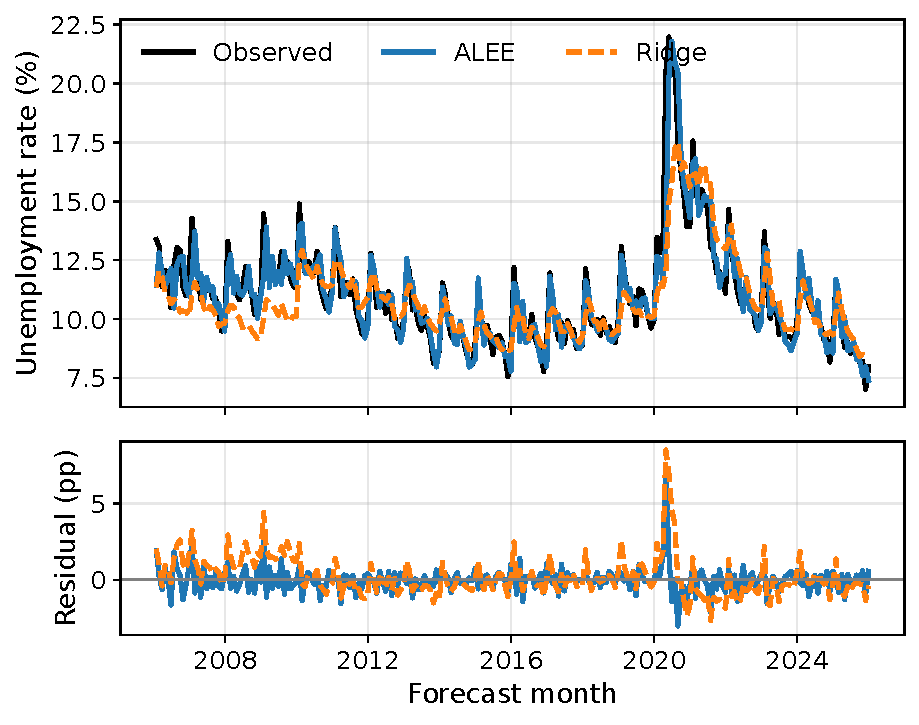
\includegraphics[width=\linewidth]{figuras/fig_pronostico_colombia.pdf}
\caption{Colombia, 240 meses de prueba (2006--2025): tasa de desempleo observada y pronósticos a un mes de ALEE y del mejor modelo del curso en ese conjunto (arriba), y residuos de ambos modelos (abajo).}
\label{fig:pronostico}
\end{figure}

\begin{figure}[H]
\centering
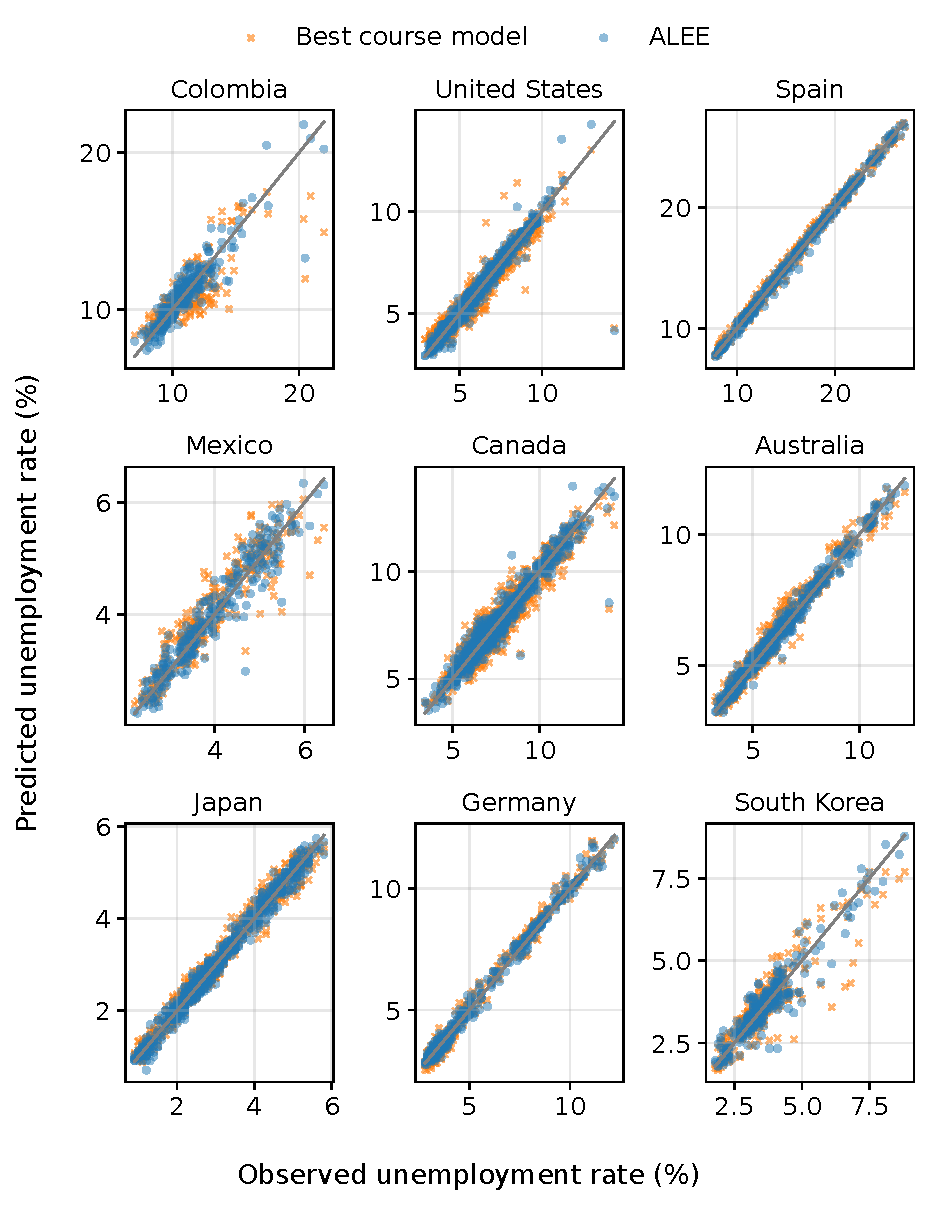
\includegraphics[width=\linewidth]{figuras/fig_predicho_observado.pdf}
\caption{Valor predicho frente a observado de ALEE y del mejor modelo del curso en cada conjunto (la línea gris es la identidad).}
\label{fig:predicho}
\end{figure}

\begin{figure}[H]
\centering
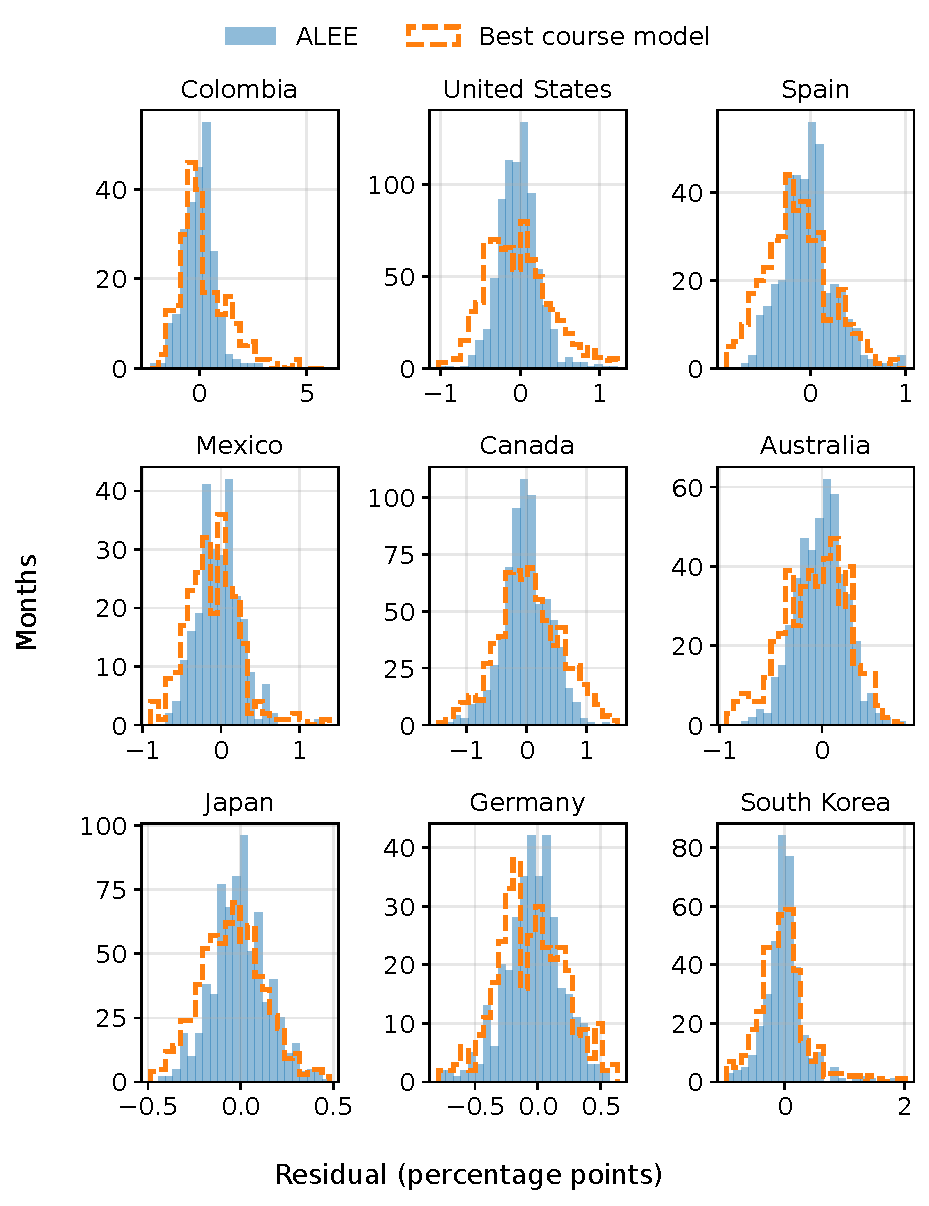
\includegraphics[width=\linewidth]{figuras/fig_residuos.pdf}
\caption{Distribución de los residuos de ALEE y del mejor modelo del curso en cada conjunto.}
\label{fig:residuos}
\end{figure}

\begin{figure}[H]
\centering
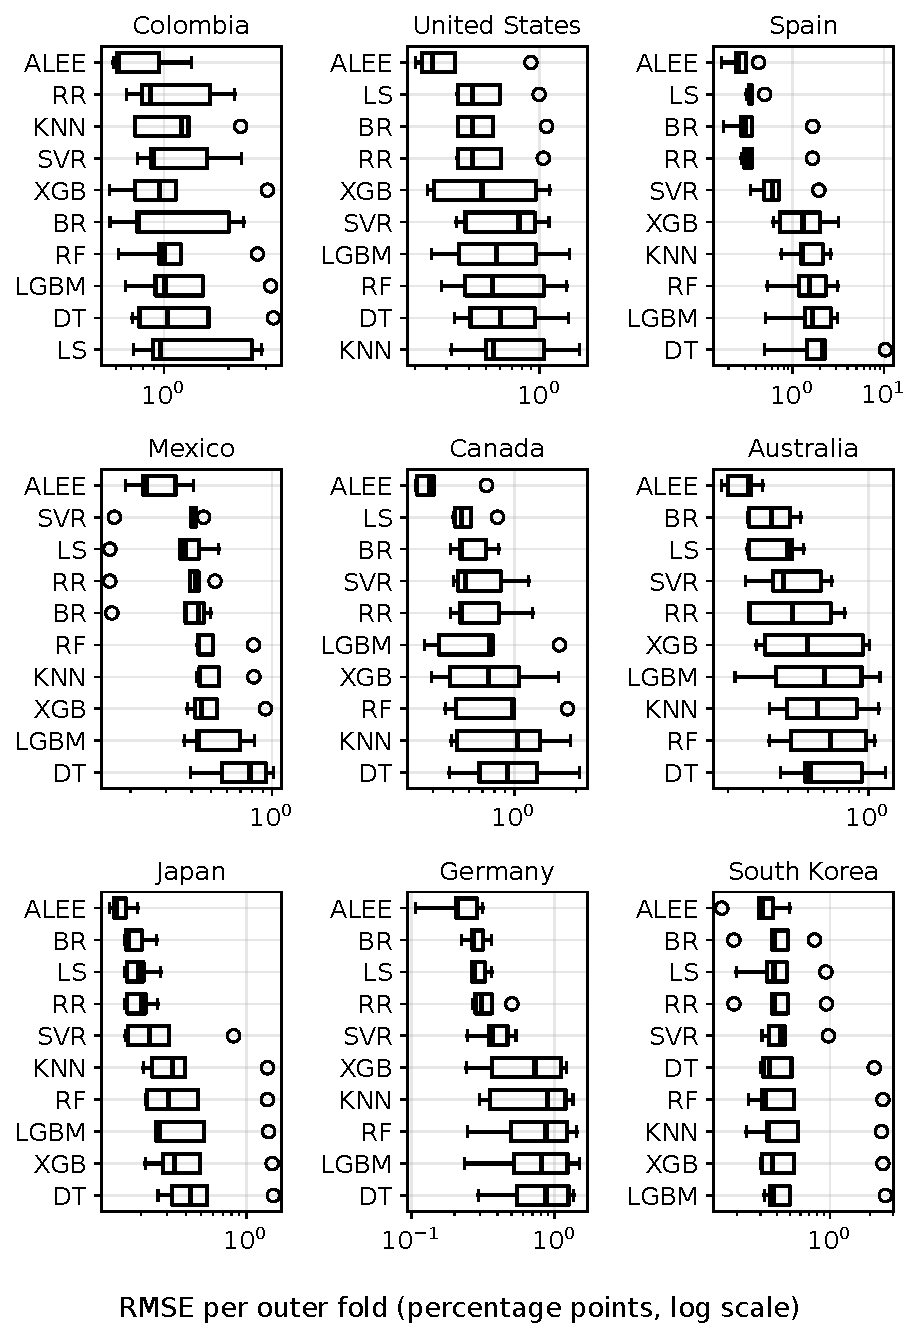
\includegraphics[width=\linewidth]{figuras/fig_rmse_pliegues.pdf}
\caption{RMSE de cada modelo en los cinco pliegues externos de cada conjunto (escala logarítmica), ordenado de menor a mayor RMSE medio. RR: Ridge; LS: Lasso; BR: regresión bayesiana; DT: árbol de decisión; RF: Random Forest; XGB: XGBoost; SVR: SVR con kernel RBF; LGBM: LightGBM.}
\label{fig:pliegues}
\end{figure}

\FloatBarrier
\subsection{Resultados de las pruebas de significancia}

La Tabla~\ref{tab:pruebas} reporta, para los nueve conjuntos, la diferencia media de pérdida con su intervalo, el estadístico y el $p$ ajustado de Diebold-Mariano y de Giacomini-White, las probabilidades de la prueba bayesiana y los tamaños de efecto. ALEE supera significativamente a los nueve modelos de comparación en los nueve conjuntos según Diebold-Mariano-HLN (el mayor $p_{\mathrm{Holm}}$ de las 81 comparaciones es 0.0074, frente a Random Forest en Colombia) y según Giacomini-White (el mayor es 0.020, frente a XGBoost en Colombia). Todos los intervalos de confianza de la diferencia de pérdida excluyen el cero. Los tamaños de efecto van de pequeños a medianos ($d$ de Cohen entre $-0.17$ y $-0.73$), y $A_{12}$ está entre 0.55 y 0.90: en la mayoría de los meses el error absoluto de ALEE es menor que el del modelo comparado. La diferencia es estadísticamente clara en todos los casos; su relevancia práctica es moderada frente a los modelos lineales y grande frente a los árboles, LightGBM y KNN.

{\tiny\setlength{\tabcolsep}{2pt}
\begin{longtable}{llcccccccc}
\caption{Pruebas de ALEE frente a cada modelo del curso en los nueve conjuntos. $\bar d$: diferencia media de pérdida cuadrática (ALEE menos el modelo; negativo favorece a ALEE) con IC del 95\,\% por \textit{bootstrap} estacionario. DM: estadístico de Diebold-Mariano-HLN; GW: estadístico de Wald de Giacomini-White condicional ($\chi^2$ con 2 g.l.); ambos con $p$ ajustado por Holm sobre los ocho modelos. $P$: probabilidades posteriores de la $t$ bayesiana correlacionada de que ALEE sea mejor, equivalente (ROPE $\pm1$\,\%) o peor. $d$: d de Cohen. $A_{12}$: probabilidad de que el error absoluto de ALEE sea menor.}\label{tab:pruebas}\\
\toprule
Conjunto & Modelo & $\bar d$ [IC 95\,\%] & DM & $p_{\mathrm{Holm}}$ & GW & $p_{\mathrm{Holm}}$ & $P$(mejor/ROPE/peor) & $d$ & $A_{12}$ \\
\midrule
\endfirsthead
\toprule
Conjunto & Modelo & $\bar d$ [IC 95\,\%] & DM & $p_{\mathrm{Holm}}$ & GW & $p_{\mathrm{Holm}}$ & $P$(mejor/ROPE/peor) & $d$ & $A_{12}$ \\
\midrule
\endhead
\bottomrule
\endfoot
Colombia & KNN & -1.130 [-2.370, -0.379] & -3.45 & 0.003 & 15.2 & 0.002 & 0.96/0.01/0.03 & -0.22 & 0.60 \\
 & Ridge & -1.058 [-1.987, -0.421] & -4.14 & $3.1\times10^{-4}$ & 22.3 & $1.0\times10^{-4}$ & 0.98/0.00/0.01 & -0.27 & 0.61 \\
 & Lasso & -2.654 [-4.782, -0.912] & -6.40 & $7.4\times10^{-9}$ & 40.8 & $1.3\times10^{-8}$ & 0.98/0.00/0.02 & -0.41 & 0.68 \\
 & Regresión bayesiana & -1.463 [-2.670, -0.506] & -5.42 & $1.2\times10^{-6}$ & 27.3 & $9.3\times10^{-6}$ & 0.89/0.01/0.10 & -0.35 & 0.60 \\
 & Árbol de decisión & -2.302 [-5.534, -0.591] & -3.48 & 0.003 & 15.2 & 0.002 & 0.97/0.00/0.03 & -0.22 & 0.65 \\
 & Random Forest & -1.476 [-3.669, -0.262] & -2.93 & 0.007 & 10.3 & 0.011 & 0.91/0.01/0.08 & -0.19 & 0.60 \\
 & XGBoost & -1.702 [-4.628, -0.127] & -2.71 & 0.007 & 7.9 & 0.020 & 0.82/0.02/0.16 & -0.17 & 0.57 \\
 & SVR (RBF) & -1.234 [-2.352, -0.507] & -4.16 & $3.1\times10^{-4}$ & 20.7 & $2.0\times10^{-4}$ & 1.00/0.00/0.00 & -0.27 & 0.61 \\
 & LightGBM & -2.149 [-5.406, -0.371] & -3.37 & 0.003 & 14.7 & 0.002 & 0.92/0.01/0.07 & -0.22 & 0.64 \\
\midrule
EE.UU. & KNN & -0.703 [-1.367, -0.284] & -8.29 & $3.6\times10^{-15}$ & 91.8 & $<10^{-15}$ & 0.96/0.00/0.04 & -0.30 & 0.71 \\
 & Ridge & -0.166 [-0.264, -0.102] & -5.92 & $1.4\times10^{-8}$ & 50.5 & $4.4\times10^{-11}$ & 0.99/0.00/0.01 & -0.21 & 0.69 \\
 & Lasso & -0.140 [-0.201, -0.093] & -6.47 & $6.8\times10^{-10}$ & 47.0 & $1.3\times10^{-10}$ & 0.98/0.00/0.02 & -0.23 & 0.68 \\
 & Regresión bayesiana & -0.171 [-0.307, -0.092] & -4.97 & $8.4\times10^{-7}$ & 38.0 & $5.6\times10^{-9}$ & 0.99/0.00/0.00 & -0.18 & 0.67 \\
 & Árbol de decisión & -0.515 [-1.081, -0.176] & -7.30 & $5.0\times10^{-12}$ & 81.3 & $<10^{-15}$ & 0.94/0.01/0.05 & -0.26 & 0.68 \\
 & Random Forest & -0.518 [-1.091, -0.183] & -6.85 & $7.5\times10^{-11}$ & 54.9 & $5.9\times10^{-12}$ & 0.95/0.01/0.05 & -0.25 & 0.69 \\
 & XGBoost & -0.297 [-0.690, -0.073] & -5.77 & $2.3\times10^{-8}$ & 49.8 & $4.5\times10^{-11}$ & 0.85/0.01/0.13 & -0.21 & 0.62 \\
 & SVR (RBF) & -0.390 [-0.637, -0.200] & -10.64 & $<10^{-15}$ & 115.9 & $<10^{-15}$ & 0.95/0.01/0.05 & -0.38 & 0.69 \\
 & LightGBM & -0.506 [-1.088, -0.162] & -7.19 & $9.0\times10^{-12}$ & 81.8 & $<10^{-15}$ & 0.91/0.01/0.08 & -0.26 & 0.67 \\
\midrule
España & KNN & -2.981 [-4.665, -1.595] & -11.63 & $<10^{-15}$ & 157.1 & $<10^{-15}$ & 1.00/0.00/0.00 & -0.59 & 0.87 \\
 & Ridge & -0.541 [-1.097, -0.126] & -9.20 & $<10^{-15}$ & 69.7 & $2.3\times10^{-15}$ & 0.73/0.02/0.25 & -0.46 & 0.62 \\
 & Lasso & -0.055 [-0.103, -0.008] & -5.67 & $2.8\times10^{-8}$ & 63.2 & $1.9\times10^{-14}$ & 0.78/0.02/0.20 & -0.29 & 0.62 \\
 & Regresión bayesiana & -0.534 [-1.098, -0.111] & -8.93 & $<10^{-15}$ & 66.5 & $7.3\times10^{-15}$ & 0.66/0.02/0.32 & -0.45 & 0.59 \\
 & Árbol de decisión & -23.769 [-52.706, -5.666] & -7.98 & $3.3\times10^{-14}$ & 79.3 & $<10^{-15}$ & 0.99/0.00/0.01 & -0.40 & 0.87 \\
 & Random Forest & -3.740 [-6.497, -1.776] & -10.03 & $<10^{-15}$ & 128.3 & $<10^{-15}$ & 1.00/0.00/0.00 & -0.50 & 0.85 \\
 & XGBoost & -3.270 [-6.188, -1.272] & -8.52 & $1.3\times10^{-15}$ & 103.0 & $<10^{-15}$ & 1.00/0.00/0.00 & -0.43 & 0.83 \\
 & SVR (RBF) & -0.916 [-1.722, -0.338] & -9.91 & $<10^{-15}$ & 117.7 & $<10^{-15}$ & 0.99/0.00/0.01 & -0.50 & 0.74 \\
 & LightGBM & -4.197 [-6.764, -2.154] & -11.25 & $<10^{-15}$ & 146.8 & $<10^{-15}$ & 0.99/0.00/0.01 & -0.57 & 0.90 \\
\midrule
México & KNN & -0.220 [-0.414, -0.094] & -5.04 & $5.3\times10^{-6}$ & 38.5 & $3.0\times10^{-8}$ & 0.95/0.01/0.04 & -0.32 & 0.68 \\
 & Ridge & -0.078 [-0.151, -0.025] & -4.31 & $6.9\times10^{-5}$ & 18.5 & $2.9\times10^{-4}$ & 0.77/0.02/0.21 & -0.27 & 0.58 \\
 & Lasso & -0.070 [-0.154, -0.018] & -3.84 & $1.6\times10^{-4}$ & 16.2 & $4.8\times10^{-4}$ & 0.75/0.02/0.23 & -0.24 & 0.55 \\
 & Regresión bayesiana & -0.079 [-0.130, -0.031] & -5.51 & $6.2\times10^{-7}$ & 27.4 & $4.5\times10^{-6}$ & 0.77/0.02/0.20 & -0.34 & 0.59 \\
 & Árbol de decisión & -0.512 [-0.795, -0.268] & -7.56 & $6.5\times10^{-12}$ & 68.0 & $1.6\times10^{-14}$ & 0.96/0.00/0.04 & -0.47 & 0.76 \\
 & Random Forest & -0.211 [-0.417, -0.081] & -4.79 & $1.4\times10^{-5}$ & 33.7 & $2.9\times10^{-7}$ & 0.94/0.01/0.06 & -0.30 & 0.67 \\
 & XGBoost & -0.249 [-0.536, -0.072] & -4.39 & $6.8\times10^{-5}$ & 29.7 & $1.8\times10^{-6}$ & 0.90/0.01/0.09 & -0.27 & 0.67 \\
 & SVR (RBF) & -0.062 [-0.113, -0.022] & -4.23 & $6.9\times10^{-5}$ & 16.7 & $4.8\times10^{-4}$ & 0.79/0.02/0.19 & -0.26 & 0.57 \\
 & LightGBM & -0.247 [-0.444, -0.100] & -5.65 & $3.4\times10^{-7}$ & 44.1 & $2.1\times10^{-9}$ & 0.93/0.01/0.06 & -0.35 & 0.70 \\
\midrule
Canadá & KNN & -1.163 [-2.006, -0.531] & -10.29 & $<10^{-15}$ & 130.7 & $<10^{-15}$ & 0.94/0.01/0.06 & -0.39 & 0.69 \\
 & Ridge & -0.397 [-0.632, -0.223] & -11.74 & $<10^{-15}$ & 128.6 & $<10^{-15}$ & 0.94/0.01/0.06 & -0.44 & 0.65 \\
 & Lasso & -0.163 [-0.219, -0.119] & -9.90 & $<10^{-15}$ & 111.3 & $<10^{-15}$ & 0.98/0.00/0.02 & -0.37 & 0.61 \\
 & Regresión bayesiana & -0.202 [-0.259, -0.153] & -10.88 & $<10^{-15}$ & 101.9 & $<10^{-15}$ & 0.97/0.01/0.03 & -0.41 & 0.62 \\
 & Árbol de decisión & -1.292 [-2.246, -0.579] & -10.13 & $<10^{-15}$ & 128.4 & $<10^{-15}$ & 0.94/0.01/0.06 & -0.38 & 0.70 \\
 & Random Forest & -0.931 [-1.702, -0.379] & -8.37 & $6.7\times10^{-16}$ & 95.7 & $<10^{-15}$ & 0.92/0.01/0.07 & -0.32 & 0.67 \\
 & XGBoost & -0.731 [-1.362, -0.263] & -8.17 & $3.1\times10^{-15}$ & 87.0 & $<10^{-15}$ & 0.84/0.01/0.15 & -0.31 & 0.63 \\
 & SVR (RBF) & -0.386 [-0.685, -0.176] & -9.36 & $<10^{-15}$ & 96.4 & $<10^{-15}$ & 0.94/0.01/0.05 & -0.35 & 0.64 \\
 & LightGBM & -0.639 [-1.296, -0.196] & -7.33 & $6.4\times10^{-13}$ & 70.9 & $4.4\times10^{-16}$ & 0.79/0.02/0.19 & -0.28 & 0.61 \\
\midrule
Australia & KNN & -0.462 [-0.743, -0.234] & -12.29 & $<10^{-15}$ & 142.4 & $<10^{-15}$ & 0.99/0.00/0.01 & -0.56 & 0.75 \\
 & Ridge & -0.203 [-0.315, -0.109] & -10.18 & $<10^{-15}$ & 95.9 & $<10^{-15}$ & 0.97/0.00/0.03 & -0.47 & 0.68 \\
 & Lasso & -0.078 [-0.112, -0.051] & -8.35 & $1.3\times10^{-15}$ & 62.4 & $5.8\times10^{-14}$ & 0.99/0.00/0.01 & -0.38 & 0.62 \\
 & Regresión bayesiana & -0.064 [-0.096, -0.040] & -7.53 & $2.6\times10^{-13}$ & 52.4 & $4.2\times10^{-12}$ & 0.99/0.00/0.01 & -0.35 & 0.60 \\
 & Árbol de decisión & -0.536 [-0.842, -0.287] & -11.72 & $<10^{-15}$ & 135.6 & $<10^{-15}$ & 0.99/0.00/0.01 & -0.54 & 0.76 \\
 & Random Forest & -0.500 [-0.786, -0.253] & -12.11 & $<10^{-15}$ & 141.8 & $<10^{-15}$ & 0.99/0.00/0.01 & -0.56 & 0.74 \\
 & XGBoost & -0.405 [-0.687, -0.176] & -10.44 & $<10^{-15}$ & 108.9 & $<10^{-15}$ & 0.95/0.00/0.04 & -0.48 & 0.69 \\
 & SVR (RBF) & -0.159 [-0.236, -0.094] & -10.29 & $<10^{-15}$ & 93.4 & $<10^{-15}$ & 0.97/0.00/0.03 & -0.47 & 0.66 \\
 & LightGBM & -0.480 [-0.845, -0.197] & -9.93 & $<10^{-15}$ & 107.4 & $<10^{-15}$ & 0.94/0.01/0.06 & -0.46 & 0.68 \\
\midrule
Japón & KNN & -0.432 [-0.889, -0.122] & -9.02 & $<10^{-15}$ & 110.8 & $<10^{-15}$ & 0.98/0.00/0.02 & -0.34 & 0.73 \\
 & Ridge & -0.018 [-0.025, -0.012] & -8.59 & $<10^{-15}$ & 67.6 & $4.2\times10^{-15}$ & 1.00/0.00/0.00 & -0.32 & 0.59 \\
 & Lasso & -0.018 [-0.026, -0.011] & -8.73 & $<10^{-15}$ & 70.0 & $2.0\times10^{-15}$ & 0.99/0.00/0.01 & -0.33 & 0.59 \\
 & Regresión bayesiana & -0.014 [-0.020, -0.009] & -7.04 & $4.6\times10^{-12}$ & 46.9 & $6.7\times10^{-11}$ & 0.94/0.01/0.05 & -0.27 & 0.58 \\
 & Árbol de decisión & -0.569 [-1.107, -0.200] & -10.00 & $<10^{-15}$ & 146.6 & $<10^{-15}$ & 1.00/0.00/0.00 & -0.38 & 0.75 \\
 & Random Forest & -0.444 [-0.903, -0.136] & -9.25 & $<10^{-15}$ & 120.7 & $<10^{-15}$ & 0.98/0.00/0.02 & -0.35 & 0.76 \\
 & XGBoost & -0.516 [-1.041, -0.164] & -9.42 & $<10^{-15}$ & 127.8 & $<10^{-15}$ & 0.98/0.00/0.01 & -0.35 & 0.79 \\
 & SVR (RBF) & -0.153 [-0.329, -0.042] & -8.10 & $4.9\times10^{-15}$ & 90.6 & $<10^{-15}$ & 0.93/0.01/0.06 & -0.31 & 0.65 \\
 & LightGBM & -0.470 [-0.946, -0.151] & -9.50 & $<10^{-15}$ & 128.3 & $<10^{-15}$ & 0.99/0.00/0.01 & -0.36 & 0.77 \\
\midrule
Alemania & KNN & -0.791 [-1.196, -0.435] & -13.59 & $<10^{-15}$ & 139.8 & $<10^{-15}$ & 0.99/0.00/0.01 & -0.73 & 0.81 \\
 & Ridge & -0.070 [-0.129, -0.029] & -7.65 & $6.1\times10^{-13}$ & 51.8 & $1.7\times10^{-11}$ & 0.86/0.01/0.12 & -0.41 & 0.64 \\
 & Lasso & -0.034 [-0.046, -0.024] & -6.25 & $2.5\times10^{-9}$ & 34.3 & $7.1\times10^{-8}$ & 0.91/0.01/0.08 & -0.34 & 0.59 \\
 & Regresión bayesiana & -0.029 [-0.039, -0.019] & -5.69 & $2.7\times10^{-8}$ & 29.8 & $3.4\times10^{-7}$ & 0.92/0.01/0.07 & -0.31 & 0.59 \\
 & Árbol de decisión & -0.855 [-1.285, -0.476] & -13.39 & $<10^{-15}$ & 138.3 & $<10^{-15}$ & 0.99/0.00/0.01 & -0.72 & 0.80 \\
 & Random Forest & -0.860 [-1.306, -0.469] & -13.59 & $<10^{-15}$ & 143.3 & $<10^{-15}$ & 0.98/0.00/0.02 & -0.73 & 0.82 \\
 & XGBoost & -0.626 [-0.979, -0.314] & -12.15 & $<10^{-15}$ & 122.2 & $<10^{-15}$ & 0.97/0.00/0.02 & -0.65 & 0.78 \\
 & SVR (RBF) & -0.110 [-0.183, -0.054] & -9.80 & $<10^{-15}$ & 78.0 & $<10^{-15}$ & 0.90/0.01/0.09 & -0.53 & 0.71 \\
 & LightGBM & -0.888 [-1.381, -0.463] & -13.08 & $<10^{-15}$ & 139.1 & $<10^{-15}$ & 0.97/0.00/0.03 & -0.70 & 0.81 \\
\midrule
Corea del Sur & KNN & -1.207 [-2.943, -0.098] & -5.13 & $2.5\times10^{-6}$ & 33.1 & $4.1\times10^{-7}$ & 0.86/0.01/0.13 & -0.27 & 0.64 \\
 & Ridge & -0.168 [-0.379, -0.030] & -5.17 & $2.5\times10^{-6}$ & 29.4 & $1.7\times10^{-6}$ & 0.86/0.02/0.13 & -0.27 & 0.60 \\
 & Lasso & -0.160 [-0.388, -0.018] & -4.43 & $2.5\times10^{-5}$ & 22.9 & $2.1\times10^{-5}$ & 0.84/0.02/0.14 & -0.23 & 0.58 \\
 & Regresión bayesiana & -0.110 [-0.259, -0.021] & -3.62 & $3.4\times10^{-4}$ & 17.7 & $1.5\times10^{-4}$ & 0.88/0.02/0.10 & -0.19 & 0.58 \\
 & Árbol de decisión & -0.928 [-2.354, -0.061] & -4.77 & $8.0\times10^{-6}$ & 27.7 & $2.9\times10^{-6}$ & 0.83/0.01/0.15 & -0.25 & 0.58 \\
 & Random Forest & -1.254 [-3.072, -0.085] & -5.13 & $2.5\times10^{-6}$ & 32.5 & $4.3\times10^{-7}$ & 0.81/0.02/0.17 & -0.27 & 0.62 \\
 & XGBoost & -1.263 [-3.088, -0.101] & -5.18 & $2.5\times10^{-6}$ & 33.3 & $4.1\times10^{-7}$ & 0.85/0.01/0.14 & -0.27 & 0.66 \\
 & SVR (RBF) & -0.193 [-0.423, -0.040] & -5.30 & $1.8\times10^{-6}$ & 34.0 & $3.2\times10^{-7}$ & 0.86/0.01/0.13 & -0.28 & 0.66 \\
 & LightGBM & -1.376 [-3.332, -0.113] & -5.27 & $1.8\times10^{-6}$ & 35.2 & $2.0\times10^{-7}$ & 0.84/0.01/0.15 & -0.28 & 0.66 \\
\end{longtable}
}

La prueba bayesiana con ROPE coincide en la dirección, pero es menos concluyente: la probabilidad posterior de que ALEE sea mejor va de 0.66 a 0.999. Los valores más bajos aparecen frente a los modelos lineales en algunos conjuntos, como la regresión bayesiana en España (0.66), justo donde Diebold-Mariano rechaza con valores $p$ muy pequeños. La discrepancia se explica por los insumos de cada prueba: Diebold-Mariano y Giacomini-White usan cientos de errores individuales, mientras que la prueba bayesiana usa solo cinco RMSE por pliegue y ajusta por la correlación entre ellos. En ningún caso la probabilidad de equivalencia práctica supera 0.03.

El conjunto de confianza de modelos ($\alpha=0.10$) conserva solo a ALEE en cuatro conjuntos (España, Australia, Japón y Alemania). En Canadá, Corea y México descarta a cuatro de los nueve modelos de comparación; en Estados Unidos, a uno; y en Colombia, donde los pliegues son pocos y muy heterogéneos, no descarta a ninguno.

Entre conjuntos (Tabla~\ref{tab:entre} y Figura~\ref{fig:cd}), la prueba de Friedman rechaza que los diez modelos sean equivalentes ($\chi^2=62.7$, $p=4.0\times10^{-10}$; Iman-Davenport $F=27.5$, $p<10^{-15}$). ALEE tiene rango 1 en los nueve conjuntos; le siguen la regresión bayesiana (3.11), Lasso (3.44), Ridge (4.00) y SVR (4.44), y quedan al final XGBoost (6.78), KNN (7.22), Random Forest (7.56), LightGBM (8.11) y el árbol de decisión (9.33). Con nueve conjuntos, las pruebas por pares tienen potencia: el Wilcoxon pareado con Holm rechaza la igualdad frente a cada uno de los nueve modelos ($p_{\mathrm{Holm}}=0.035$, el mínimo posible con nueve conjuntos), y el signed-rank bayesiano da una probabilidad superior a 0.999 de que ALEE sea mejor que cada uno. El post-hoc de Conover con Holm la rechaza frente a ocho de los nueve; frente a la regresión bayesiana, el segundo mejor modelo, queda en $p_{\mathrm{Holm}}=0.071$.

\begin{table}[H]
\centering
\caption{Comparación entre los nueve conjuntos: rango medio según el RMSE medio de pliegues (1 = mejor), número de conjuntos en que ALEE tiene menor RMSE, Wilcoxon pareado y post-hoc de Conover frente a ALEE, ambos con Holm, y probabilidades del signed-rank bayesiano (ALEE mejor/equivalente/peor).}
\label{tab:entre}
\small
\resizebox{\textwidth}{!}{\begin{tabular}{lccccc}
\toprule
Modelo & Rango medio & Conjuntos en que ALEE gana & Wilcoxon $p_{\mathrm{Holm}}$ & Conover $p_{\mathrm{Holm}}$ & $P$(mejor/ROPE/peor) \\
\midrule
ALEE & 1.00 & --- & --- & --- & --- \\
\midrule
Regresión bayesiana & 3.11 & 9/9 & 0.035 & 0.071 & 1.000/0.000/0.000 \\
Lasso & 3.44 & 9/9 & 0.035 & 0.020 & 1.000/0.000/0.000 \\
Ridge & 4.00 & 9/9 & 0.035 & 0.002 & 1.000/0.000/0.000 \\
SVR (RBF) & 4.44 & 9/9 & 0.035 & $2.3\times10^{-4}$ & 1.000/0.000/0.000 \\
XGBoost & 6.78 & 9/9 & 0.035 & $5.2\times10^{-10}$ & 1.000/0.000/0.000 \\
KNN & 7.22 & 9/9 & 0.035 & $3.9\times10^{-11}$ & 1.000/0.000/0.000 \\
Random Forest & 7.56 & 9/9 & 0.035 & $5.5\times10^{-12}$ & 1.000/0.000/0.000 \\
LightGBM & 8.11 & 9/9 & 0.035 & $2.1\times10^{-13}$ & 1.000/0.000/0.000 \\
Árbol de decisión & 9.33 & 9/9 & 0.035 & $1.8\times10^{-16}$ & 1.000/0.000/0.000 \\
\bottomrule
\end{tabular}}
\end{table}

\begin{figure}[H]
\centering
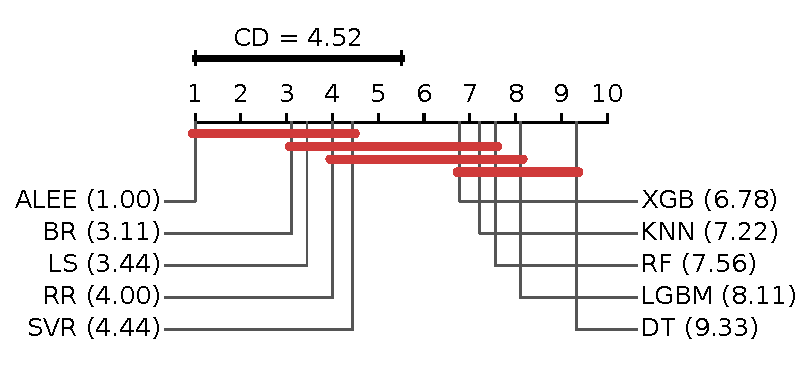
\includegraphics[width=\linewidth]{figuras/fig_cd.pdf}
\caption{Diagrama de diferencia crítica de Nemenyi ($\alpha=0.05$) con los nueve conjuntos como bloques. Las barras unen modelos cuya diferencia de rango medio es menor que la diferencia crítica. Abreviaturas como en la Figura~\ref{fig:pliegues}.}
\label{fig:cd}
\end{figure}

En síntesis, ALEE supera significativamente a los ocho modelos del curso y a LightGBM en cada uno de los nueve conjuntos, con las tres pruebas en la misma dirección, y también entre conjuntos. Esto responde la pregunta de investigación de forma afirmativa: ALEE pronostica mejor que cada modelo del curso, con efectos no despreciables ($|d|\ge0.17$).

\FloatBarrier
\subsection{Resultados del estudio de ablación}

La Tabla~\ref{tab:ablacion} resume el RMSE de cada variante, la Tabla~\ref{tab:ablacion_completa} reporta las cinco métricas y la Figura~\ref{fig:ablacion} lo muestra gráficamente. Con ellas se contrastan las cinco hipótesis de la Sección~\ref{sec:ablacion}. \textbf{H1 se confirma en siete de los nueve conjuntos}: el promedio simple es significativamente peor en todos salvo en Alemania, donde es peor pero sin significancia, y en Japón, donde es algo mejor (0.142 frente a 0.149; $p_{\mathrm{Holm}}=0.060$). \textbf{H2 se confirma solo en dos conjuntos}: quitar la localización empeora el error de forma significativa en México ($p_{\mathrm{Holm}}=0.019$) y en Japón ($p_{\mathrm{Holm}}=0.0026$); en los otros siete no hay diferencia significativa, y en Colombia y Alemania la versión sin localización tiene incluso menor RMSE. \textbf{H3 se confirma en dos conjuntos}: la regularización adaptativa mejora de forma significativa en Canadá y Japón, aunque por menos de 2\,\%. \textbf{H4 se refuta}: el previo uniforme no difiere significativamente del global en ningún conjunto. \textbf{H5 se confirma en parte}: la persistencia y el núcleo por separado son significativamente peores en los nueve conjuntos, y el experto estacional solo es significativamente peor en Canadá, Australia y Japón (por ejemplo, 0.513 frente a 0.437 en Canadá), pero no se distingue de ALEE en los otros seis. Donde las diferencias son significativas, las cinco métricas apuntan en la misma dirección; donde no lo son, las métricas a veces discrepan en el signo, lo que confirma que esas diferencias son despreciables.

\begin{table}[H]
\centering
\caption{Ablación: RMSE medio de pliegues de cada variante. $^{\dagger}$: la variante es significativamente peor que ALEE completo (Diebold-Mariano-HLN, $p$ ajustado por Holm dentro de cada conjunto $<0.05$).}
\label{tab:ablacion}
\scriptsize
\setlength{\tabcolsep}{3pt}
\resizebox{\textwidth}{!}{\begin{tabular}{lccccccccc}
\toprule
Variante & Colombia & EE.UU. & España & México & Canadá & Australia & Japón & Alemania & Corea del Sur \\
\midrule
ALEE completo & 0.817 & 0.380 & 0.280 & 0.281 & 0.437 & 0.240 & 0.149 & 0.226 & 0.325 \\
\midrule
Sin localización & 0.797 & 0.382 & 0.280 & 0.285$^{\dagger}$ & 0.438 & 0.240 & 0.154$^{\dagger}$ & 0.222 & 0.328 \\
Sin $\lambda$ adaptativa & 0.825 & 0.383 & 0.280 & 0.280 & 0.439$^{\dagger}$ & 0.241 & 0.151$^{\dagger}$ & 0.223 & 0.325 \\
Previo uniforme & 0.822 & 0.382 & 0.281 & 0.282 & 0.437 & 0.239 & 0.148 & 0.223 & 0.328 \\
Promedio simple & 1.035$^{\dagger}$ & 0.444$^{\dagger}$ & 0.304$^{\dagger}$ & 0.310$^{\dagger}$ & 0.469$^{\dagger}$ & 0.279$^{\dagger}$ & 0.142 & 0.244 & 0.348$^{\dagger}$ \\
Solo persistencia & 1.273$^{\dagger}$ & 0.536$^{\dagger}$ & 0.325$^{\dagger}$ & 0.361$^{\dagger}$ & 0.591$^{\dagger}$ & 0.343$^{\dagger}$ & 0.167$^{\dagger}$ & 0.271$^{\dagger}$ & 0.393$^{\dagger}$ \\
Solo núcleo & 1.252$^{\dagger}$ & 0.532$^{\dagger}$ & 0.330$^{\dagger}$ & 0.362$^{\dagger}$ & 0.577$^{\dagger}$ & 0.339$^{\dagger}$ & 0.165$^{\dagger}$ & 0.270$^{\dagger}$ & 0.387$^{\dagger}$ \\
Solo estacional & 0.780 & 0.391 & 0.279 & 0.283 & 0.513$^{\dagger}$ & 0.251$^{\dagger}$ & 0.174$^{\dagger}$ & 0.231 & 0.318 \\
\bottomrule
\end{tabular}}
\end{table}

{\scriptsize\setlength{\tabcolsep}{3pt}
\begin{longtable}{llcccccc}
\caption{Ablación con todas las métricas (media entre pliegues) y $p$ de Diebold-Mariano-HLN frente a ALEE completo, ajustado por Holm dentro de cada conjunto.}\label{tab:ablacion_completa}\\
\toprule
Conjunto & Variante & RMSE & MAE & MAPE (\%) & $R^2$ & MASE & DM $p_{\mathrm{Holm}}$ \\
\midrule
\endfirsthead
\toprule
Conjunto & Variante & RMSE & MAE & MAPE (\%) & $R^2$ & MASE & DM $p_{\mathrm{Holm}}$ \\
\midrule
\endhead
\bottomrule
\endfoot
Colombia & ALEE completo & 0.817 & 0.586 & 5.15 & 0.660 & 0.550 & --- \\
 & Sin localización & 0.797 & 0.567 & 4.98 & 0.674 & 0.535 & 1.000 \\
 & Sin $\lambda$ adaptativa & 0.825 & 0.587 & 5.16 & 0.644 & 0.552 & 1.000 \\
 & Previo uniforme & 0.822 & 0.586 & 5.15 & 0.659 & 0.551 & 1.000 \\
 & Promedio simple & 1.035 & 0.745 & 6.45 & 0.464 & 0.710 & $2.2\times10^{-5}$ \\
 & Solo persistencia & 1.273 & 0.905 & 7.82 & 0.163 & 0.862 & $2.6\times10^{-7}$ \\
 & Solo núcleo & 1.252 & 0.888 & 7.68 & 0.190 & 0.845 & $4.8\times10^{-7}$ \\
 & Solo estacional & 0.780 & 0.564 & 4.98 & 0.702 & 0.532 & 0.562 \\
\midrule
EE.UU. & ALEE completo & 0.380 & 0.210 & 3.65 & 0.901 & 0.220 & --- \\
 & Sin localización & 0.382 & 0.211 & 3.67 & 0.900 & 0.220 & 0.888 \\
 & Sin $\lambda$ adaptativa & 0.383 & 0.211 & 3.66 & 0.900 & 0.221 & 0.888 \\
 & Previo uniforme & 0.382 & 0.210 & 3.63 & 0.901 & 0.219 & 0.888 \\
 & Promedio simple & 0.444 & 0.263 & 4.53 & 0.874 & 0.273 & $5.2\times10^{-6}$ \\
 & Solo persistencia & 0.536 & 0.340 & 5.89 & 0.825 & 0.352 & $9.6\times10^{-14}$ \\
 & Solo núcleo & 0.532 & 0.341 & 5.95 & 0.828 & 0.352 & $8.3\times10^{-13}$ \\
 & Solo estacional & 0.391 & 0.220 & 3.85 & 0.897 & 0.231 & 0.132 \\
\midrule
España & ALEE completo & 0.280 & 0.218 & 1.49 & 0.989 & 0.134 & --- \\
 & Sin localización & 0.280 & 0.218 & 1.49 & 0.989 & 0.134 & 1.000 \\
 & Sin $\lambda$ adaptativa & 0.280 & 0.218 & 1.48 & 0.989 & 0.134 & 1.000 \\
 & Previo uniforme & 0.281 & 0.219 & 1.49 & 0.989 & 0.134 & 1.000 \\
 & Promedio simple & 0.304 & 0.238 & 1.61 & 0.987 & 0.145 & $1.9\times10^{-6}$ \\
 & Solo persistencia & 0.325 & 0.252 & 1.72 & 0.984 & 0.154 & $2.6\times10^{-8}$ \\
 & Solo núcleo & 0.330 & 0.260 & 1.76 & 0.984 & 0.158 & $9.4\times10^{-11}$ \\
 & Solo estacional & 0.279 & 0.216 & 1.47 & 0.989 & 0.132 & 1.000 \\
\midrule
México & ALEE completo & 0.281 & 0.220 & 5.57 & 0.628 & 0.490 & --- \\
 & Sin localización & 0.285 & 0.223 & 5.67 & 0.609 & 0.496 & 0.019 \\
 & Sin $\lambda$ adaptativa & 0.280 & 0.218 & 5.52 & 0.631 & 0.486 & 0.765 \\
 & Previo uniforme & 0.282 & 0.220 & 5.59 & 0.627 & 0.491 & 0.735 \\
 & Promedio simple & 0.310 & 0.233 & 5.84 & 0.562 & 0.519 & 0.002 \\
 & Solo persistencia & 0.361 & 0.277 & 7.04 & 0.413 & 0.618 & $1.3\times10^{-7}$ \\
 & Solo núcleo & 0.362 & 0.278 & 7.06 & 0.405 & 0.620 & $5.6\times10^{-8}$ \\
 & Solo estacional & 0.283 & 0.222 & 5.68 & 0.606 & 0.494 & 0.765 \\
\midrule
Canadá & ALEE completo & 0.437 & 0.313 & 4.23 & 0.880 & 0.354 & --- \\
 & Sin localización & 0.438 & 0.315 & 4.28 & 0.877 & 0.356 & 1.000 \\
 & Sin $\lambda$ adaptativa & 0.439 & 0.315 & 4.26 & 0.879 & 0.356 & $1.7\times10^{-5}$ \\
 & Previo uniforme & 0.437 & 0.312 & 4.22 & 0.877 & 0.353 & 1.000 \\
 & Promedio simple & 0.469 & 0.336 & 4.50 & 0.860 & 0.381 & $8.6\times10^{-5}$ \\
 & Solo persistencia & 0.591 & 0.427 & 5.68 & 0.793 & 0.482 & $<10^{-15}$ \\
 & Solo núcleo & 0.577 & 0.417 & 5.55 & 0.800 & 0.470 & $<10^{-15}$ \\
 & Solo estacional & 0.513 & 0.387 & 5.34 & 0.842 & 0.433 & $3.4\times10^{-12}$ \\
\midrule
Australia & ALEE completo & 0.240 & 0.193 & 3.26 & 0.914 & 0.226 & --- \\
 & Sin localización & 0.240 & 0.193 & 3.24 & 0.913 & 0.225 & 1.000 \\
 & Sin $\lambda$ adaptativa & 0.241 & 0.193 & 3.24 & 0.913 & 0.225 & 1.000 \\
 & Previo uniforme & 0.239 & 0.192 & 3.23 & 0.914 & 0.224 & 1.000 \\
 & Promedio simple & 0.279 & 0.219 & 3.55 & 0.886 & 0.250 & $7.0\times10^{-6}$ \\
 & Solo persistencia & 0.343 & 0.271 & 4.38 & 0.820 & 0.307 & $1.2\times10^{-14}$ \\
 & Solo núcleo & 0.339 & 0.268 & 4.36 & 0.824 & 0.304 & $2.1\times10^{-14}$ \\
 & Solo estacional & 0.251 & 0.203 & 3.45 & 0.902 & 0.238 & $1.5\times10^{-5}$ \\
\midrule
Japón & ALEE completo & 0.149 & 0.118 & 4.50 & 0.884 & 0.554 & --- \\
 & Sin localización & 0.154 & 0.121 & 4.64 & 0.876 & 0.567 & 0.003 \\
 & Sin $\lambda$ adaptativa & 0.151 & 0.119 & 4.56 & 0.882 & 0.560 & $1.5\times10^{-5}$ \\
 & Previo uniforme & 0.148 & 0.117 & 4.48 & 0.887 & 0.550 & 0.297 \\
 & Promedio simple & 0.142 & 0.113 & 4.19 & 0.898 & 0.530 & 0.060 \\
 & Solo persistencia & 0.167 & 0.129 & 4.90 & 0.860 & 0.607 & 0.001 \\
 & Solo núcleo & 0.165 & 0.129 & 4.90 & 0.864 & 0.608 & 0.003 \\
 & Solo estacional & 0.174 & 0.133 & 5.12 & 0.832 & 0.625 & $1.4\times10^{-11}$ \\
\midrule
Alemania & ALEE completo & 0.226 & 0.180 & 3.53 & 0.867 & 0.252 & --- \\
 & Sin localización & 0.222 & 0.178 & 3.47 & 0.869 & 0.248 & 0.764 \\
 & Sin $\lambda$ adaptativa & 0.223 & 0.179 & 3.51 & 0.869 & 0.251 & 0.738 \\
 & Previo uniforme & 0.223 & 0.179 & 3.50 & 0.869 & 0.250 & 0.764 \\
 & Promedio simple & 0.244 & 0.197 & 3.70 & 0.862 & 0.276 & 0.075 \\
 & Solo persistencia & 0.271 & 0.219 & 4.02 & 0.836 & 0.306 & $3.4\times10^{-5}$ \\
 & Solo núcleo & 0.270 & 0.220 & 4.05 & 0.837 & 0.307 & $2.0\times10^{-5}$ \\
 & Solo estacional & 0.231 & 0.184 & 3.67 & 0.849 & 0.258 & 0.764 \\
\midrule
Corea del Sur & ALEE completo & 0.325 & 0.234 & 6.47 & 0.709 & 0.477 & --- \\
 & Sin localización & 0.328 & 0.235 & 6.51 & 0.705 & 0.482 & 0.152 \\
 & Sin $\lambda$ adaptativa & 0.325 & 0.233 & 6.47 & 0.707 & 0.477 & 0.928 \\
 & Previo uniforme & 0.328 & 0.236 & 6.52 & 0.709 & 0.485 & 0.632 \\
 & Promedio simple & 0.348 & 0.249 & 6.84 & 0.667 & 0.514 & $5.8\times10^{-5}$ \\
 & Solo persistencia & 0.393 & 0.282 & 7.74 & 0.559 & 0.573 & $5.1\times10^{-9}$ \\
 & Solo núcleo & 0.387 & 0.279 & 7.63 & 0.577 & 0.568 & $2.9\times10^{-8}$ \\
 & Solo estacional & 0.318 & 0.232 & 6.51 & 0.718 & 0.470 & 0.928 \\
\end{longtable}
}

\begin{figure}[H]
\centering
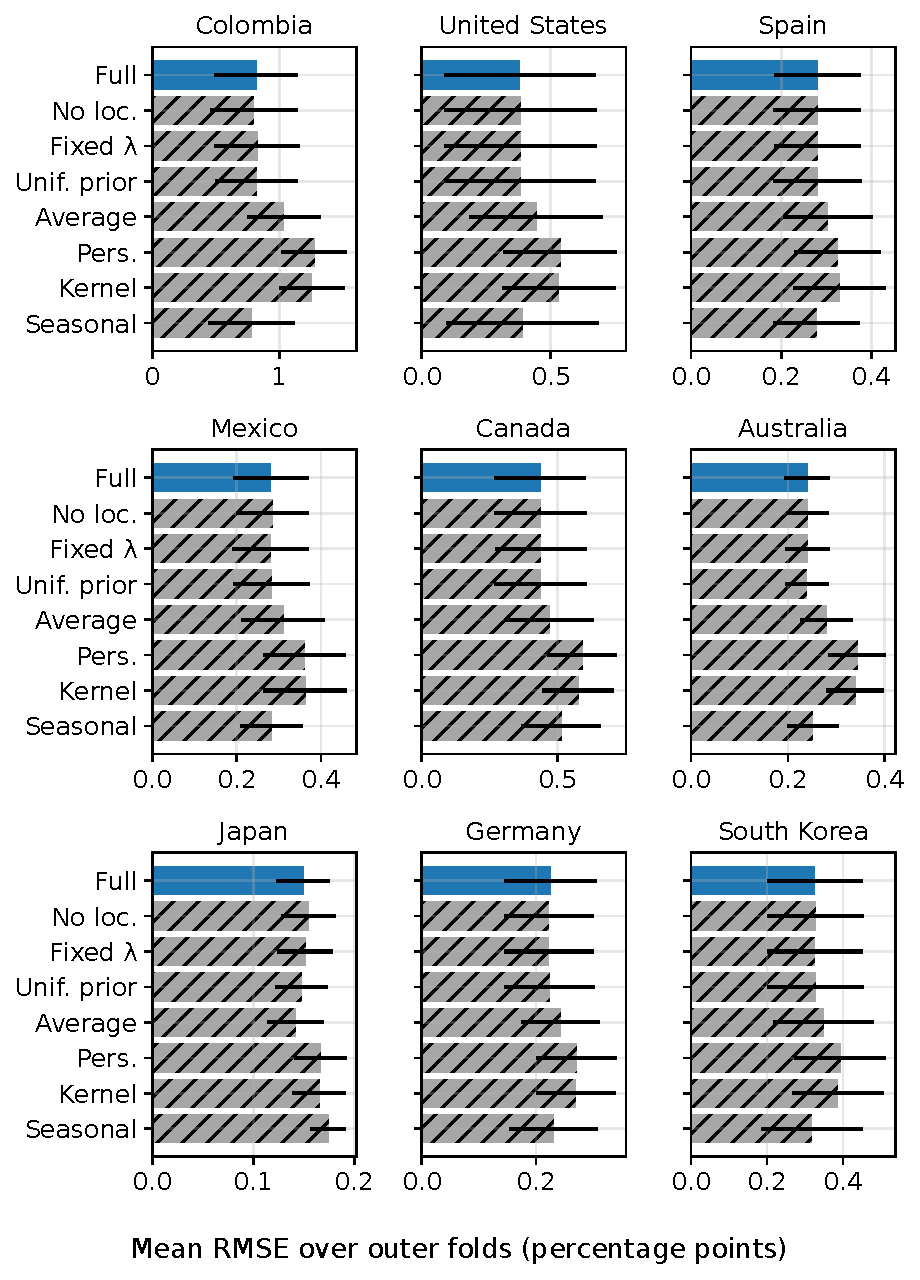
\includegraphics[width=\linewidth]{figuras/fig_ablacion.pdf}
\caption{RMSE medio de pliegues de cada variante de la ablación (barras de error: desviación estándar entre pliegues). Full: ALEE completo; No loc.: sin localización; Fixed $\lambda$: sin regularización adaptativa; Unif. prior: previo uniforme; Average: promedio simple; Pers., Kernel y Seasonal: cada experto por separado.}
\label{fig:ablacion}
\end{figure}

\FloatBarrier
\subsection{Sensibilidad y robustez}

La Tabla~\ref{tab:semillas} resume la variación entre semillas en los cuatro conjuntos originales. La de ALEE es menor que el ROPE del 1\,\% (desviación estándar de 0.003\,pp o menos), mucho menor que la de Random Forest (0.027), XGBoost (0.072) y LightGBM (0.079) en Colombia, y ninguna semilla de esos modelos se acerca al RMSE de ALEE. La ventaja de ALEE no depende de la semilla.

\begin{table}[H]
\centering
\caption{Variación del RMSE medio de pliegues entre semillas del optimizador.}
\label{tab:semillas}
\small
\begin{tabular}{llcccc}
\toprule
Conjunto & Modelo (semillas) & Media & Desv. & Mín. & Máx. \\
\midrule
Colombia & LightGBM (42--51) & 1.512 & 0.079 & 1.412 & 1.629 \\
Colombia & Random Forest (42--51) & 1.279 & 0.027 & 1.242 & 1.320 \\
Colombia & XGBoost (42--51) & 1.300 & 0.072 & 1.228 & 1.478 \\
Colombia & ALEE (42--46) & 0.821 & 0.003 & 0.817 & 0.824 \\
EE.UU. & ALEE (42--46) & 0.381 & 0.001 & 0.380 & 0.382 \\
España & ALEE (42--46) & 0.280 & 0.000 & 0.280 & 0.281 \\
México & ALEE (42--46) & 0.280 & 0.001 & 0.279 & 0.281 \\
\bottomrule
\end{tabular}
\end{table}

El mapa de sensibilidad (Figura~\ref{fig:sensibilidad}) muestra que, con $\lambda$ grande, el RMSE se estabiliza en torno a 0.792 en Colombia y 0.379 en Estados Unidos, para cualquier ancho de banda; con $\lambda$ y $h$ pequeños, el error crece hasta 0.914 en Colombia. En toda la rejilla el error de ALEE sigue muy por debajo del de cualquier modelo de comparación. El RMSE con hiperparámetros ajustados (0.817) es algo peor que esa meseta: la validación interna, con pliegues cortos, tiende a elegir regularizaciones débiles y vidas medias cortas (de 6 a 9 meses en Colombia). Esta observación es exploratoria y no se usa para cambiar los hiperparámetros, porque hacerlo sería ajustar con los datos de evaluación.

\begin{figure}[H]
\centering
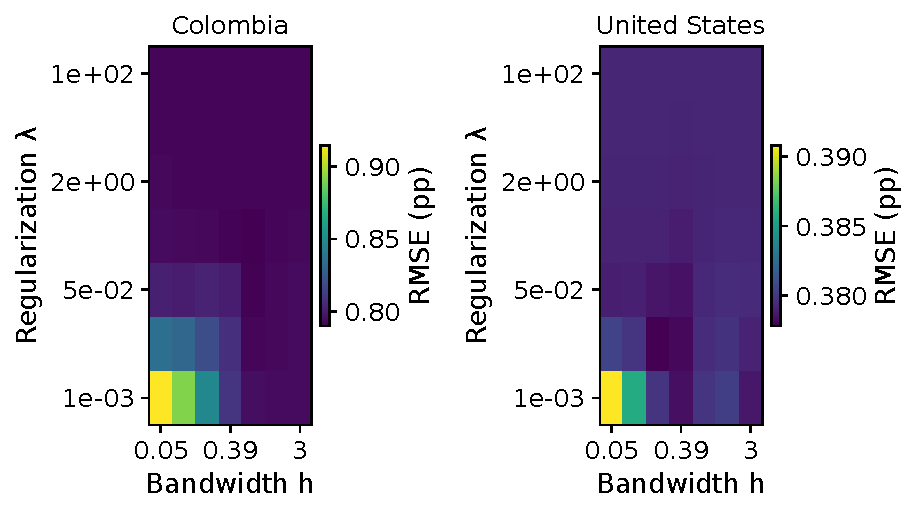
\includegraphics[width=\linewidth]{figuras/fig_sensibilidad.pdf}
\caption{RMSE medio de pliegues de ALEE con hiperparámetros fijos en una rejilla de ancho de banda $h$ y regularización $\lambda$ (vida media de 60 meses), en Colombia y Estados Unidos.}
\label{fig:sensibilidad}
\end{figure}

La curva de aprendizaje (Figura~\ref{fig:curva}) usa un periodo de prueba fijo, los últimos 156 meses de Estados Unidos (2013--2026, que incluyen 2020). ALEE alcanza su mejor error con solo 60 meses de entrenamiento (0.894) y no mejora con más datos (0.907 con 777 meses). Ridge, en cambio, necesita mucha historia: su RMSE baja de 1.81 a 1.03, y aun con toda la serie queda por encima de ALEE. ALEE funciona, por lo tanto, con series cortas, pero no aprovecha la información adicional.

\begin{figure}[H]
\centering
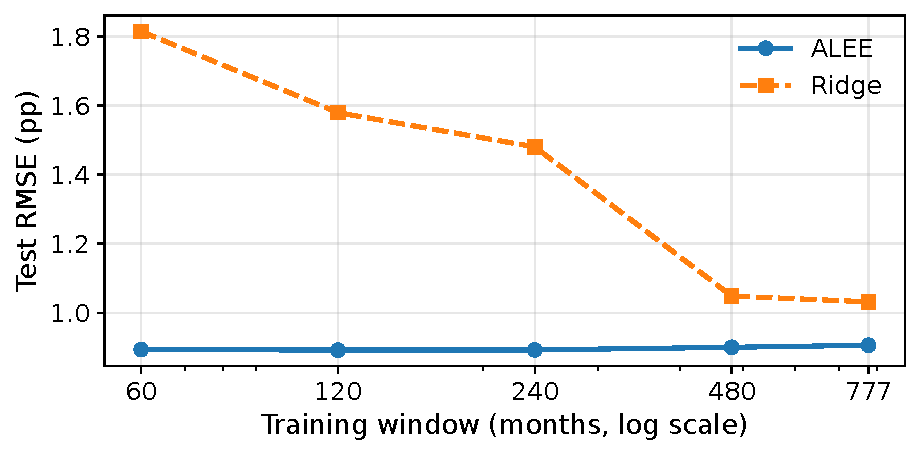
\includegraphics[width=\linewidth]{figuras/fig_curva_aprendizaje.pdf}
\caption{Curva de aprendizaje en Estados Unidos: RMSE en un periodo de prueba fijo (últimos 156 meses) según la longitud de la ventana de entrenamiento.}
\label{fig:curva}
\end{figure}

\FloatBarrier
\subsection{Costo computacional}

La Tabla~\ref{tab:costo} reporta el costo de entrenar y predecir en el último pliegue de Colombia (239 meses de entrenamiento y 48 de prueba), con los hiperparámetros elegidos en ese pliegue, cada modelo en un proceso independiente. ALEE tarda 0.69\,s en entrenar y 0.54\,s en predecir 48 meses, porque resuelve un problema convexo por cada mes pronosticado, y su proceso usa 27\,MB adicionales de memoria. Es unas 350 veces más lento que Ridge y el doble que Random Forest, aunque en términos absolutos sigue siendo trivial para un pronóstico mensual. La memoria de XGBoost (102\,MB) refleja sobre todo la inicialización de su biblioteca nativa. La validación anidada completa de ALEE es la más costosa del estudio (unos 11 minutos en Estados Unidos, frente a menos de 2 minutos de cualquier modelo de comparación), porque el historial de errores de los expertos crece de forma cúbica con la longitud de la serie. Dada la reducción del error de 21\,\% a 33\,\%, el costo adicional se justifica.

\begin{table}[H]
\centering
\caption{Costo computacional en el último pliegue de Colombia, con los hiperparámetros elegidos en ese pliegue: mediana de tres repeticiones del tiempo de entrenamiento y de inferencia (48 meses), memoria adicional del proceso y número de parámetros aprendidos o almacenados.}
\label{tab:costo}
\small
\begin{tabular}{lcccc}
\toprule
Modelo & Entrenamiento (s) & Inferencia (s) & Memoria (MB) & Parámetros \\
\midrule
KNN & 0.002 & 0.0046 & 1.00 & 4302 \\
Ridge & 0.002 & 0.0004 & 0.37 & 18 \\
Lasso & 0.002 & 0.0004 & 0.18 & 18 \\
Árbol de decisión & 0.004 & 0.0003 & 0.17 & 77 \\
Random Forest & 0.334 & 0.0230 & 0.75 & 36808 \\
XGBoost & 0.050 & 0.0014 & 102.02 & 615 \\
Regresión bayesiana & 0.002 & 0.0007 & 0.58 & 18 \\
SVR (RBF) & 0.011 & 0.0037 & 0.44 & 4285 \\
LightGBM & 0.027 & 0.0013 & 10.21 & 1343 \\
ALEE & 0.694 & 0.5435 & 27.20 & 1021 \\
\bottomrule
\end{tabular}
\end{table}

\FloatBarrier
\subsection{Interpretabilidad y análisis de errores}

La importancia por permutación de ALEE en el último pliegue de Colombia (Figura~\ref{fig:importancia}) se concentra en tres variables: el último valor observado (permutarlo aumenta el RMSE en 1.38\,pp) y las dos componentes del mes (0.79 y 0.52\,pp). Las demás, incluidos los tres indicadores de área, tienen importancia prácticamente nula (menos de 0.001\,pp). Esto concuerda con el dominio: a un mes, el desempleo se explica sobre todo por su nivel actual y por su estacionalidad. Como el seno y el coseno del mes están correlacionados, sus importancias por separado deben leerse en conjunto.

\begin{figure}[H]
\centering
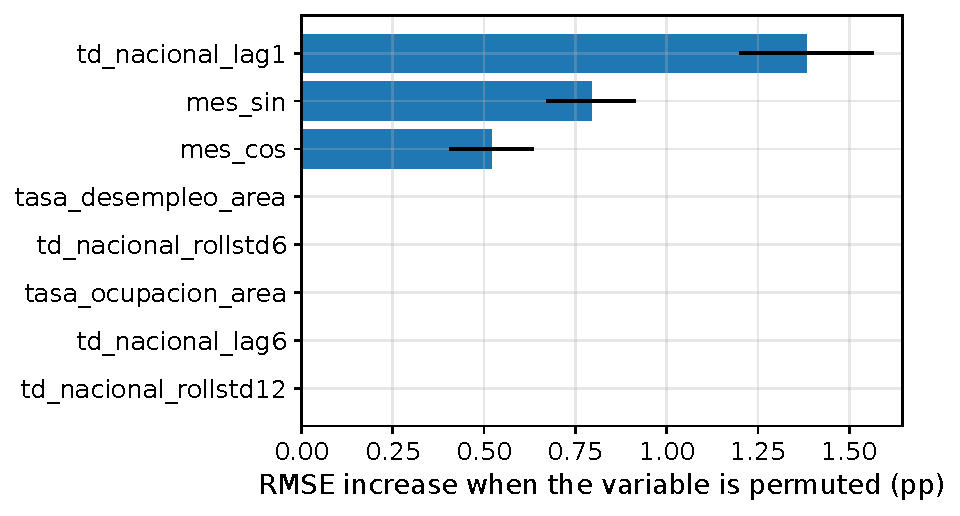
\includegraphics[width=\linewidth]{figuras/fig_importancia.pdf}
\caption{Importancia por permutación de las ocho variables principales para ALEE (Colombia, último pliegue externo; 20 permutaciones, barras de error: desviación estándar).}
\label{fig:importancia}
\end{figure}

Los pesos de la combinación (Figura~\ref{fig:pesos}) saltan entre expertos en los dos primeros pliegues de Colombia (2006--2013), cuando la historia de errores es corta: el peso medio del experto estacional es 0.55 y 0.76 en esos pliegues. Desde 2014 se concentran casi por completo en él (0.96 a 1.00 en promedio), incluso durante 2020. En Colombia, ALEE se comporta en la práctica como su experto estacional.

\begin{figure}[H]
\centering
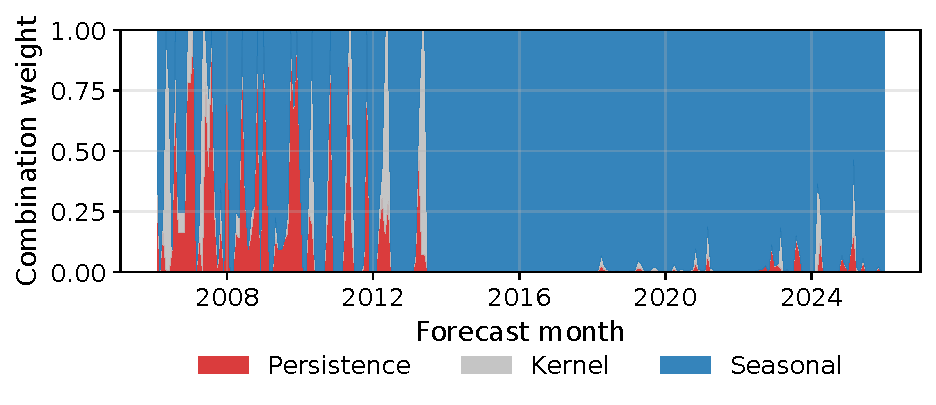
\includegraphics[width=\linewidth]{figuras/fig_pesos.pdf}
\caption{Pesos de los tres expertos de ALEE en cada mes pronosticado de Colombia.}
\label{fig:pesos}
\end{figure}

El error por tercil de volatilidad reciente (Figura~\ref{fig:errores}) muestra que ALEE tiene el menor error en los tres terciles de los nueve conjuntos (27 de 27). En Colombia, la mayor ventaja relativa aparece con volatilidad media (0.653 frente a 1.000 de Ridge). El tercil de volatilidad baja concentra el mayor error de ALEE en Colombia (1.120) porque el choque de 2020 llegó tras meses tranquilos: ningún estado observado anticipa un salto sin precedentes, y ese es el principal modo de fallo del modelo.

\begin{figure}[H]
\centering
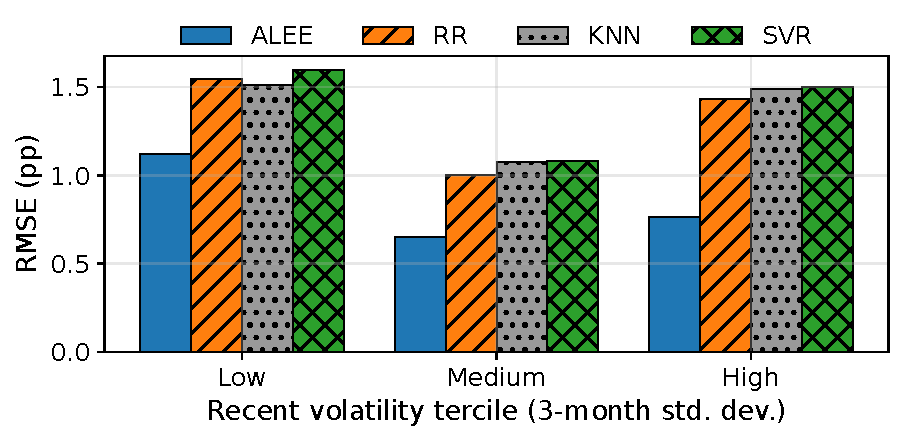
\includegraphics[width=\linewidth]{figuras/fig_errores_regimen.pdf}
\caption{RMSE de ALEE y de los tres mejores modelos de comparación en Colombia, según el tercil de volatilidad reciente (desviación estándar de los últimos tres meses). Abreviaturas como en la Figura~\ref{fig:pliegues}.}
\label{fig:errores}
\end{figure}

% ============================================================
% 4. DISCUSIÓN
% ============================================================
\FloatBarrier
\subsection{Discusión y limitaciones}
\label{sec:discusion}

Los resultados sugieren que ALEE pronostica la tasa de desempleo a un mes mejor que los modelos de regresión del curso y que LightGBM, de forma consistente en nueve países con mercados laborales distintos y en las cinco métricas. La ablación explica de dónde viene esa ventaja. La mayor parte proviene de los expertos: el experto estacional incorpora directamente la estructura que los modelos genéricos tienen que aprender a partir de pocas observaciones ---el nivel actual más el cambio típico del mes---, lo que coincide con lo observado en comparaciones a gran escala, donde los métodos que codifican la estructura temporal suelen superar a los modelos genéricos en series univariadas \cite{makridakis2018,makridakis2020}. La combinación aprendida añade valor en la mayoría de los conjuntos (supera al promedio simple en siete de nueve) y, en Canadá, Australia y Japón, también al experto estacional por sí solo. La localización por estado, en cambio, que era la idea central del modelo, solo aporta de forma significativa en México y Japón: el cambio de ganador según el régimen existe entre los modelos genéricos, pero no tanto entre los expertos de ALEE, porque el estacional domina en casi todos los regímenes \cite{elliotttimmermann2005,timmermann2006}.

Este trabajo tiene varias limitaciones. Primera, nueve conjuntos dan una potencia moderada a las pruebas entre conjuntos (la guía recomienda diez o más para Friedman): el Wilcoxon alcanza su mínimo posible, pero el Conover no distingue a ALEE de la regresión bayesiana. Segunda, la prueba bayesiana con ROPE supone particiones intercambiables y aquí se aplica sobre cinco pliegues temporales dependientes, por lo que sus probabilidades son orientativas. Tercera, en Colombia se evaluaron diez iteraciones de diseño sobre los mismos 240 meses (Sección~\ref{sec:preregistro}), lo que puede volver optimista el resultado de ALEE en ese conjunto; los ocho conjuntos adicionales, evaluados una sola vez con el modelo congelado, son por eso la evidencia más confiable. Cuarta, varias piezas del análisis se agregaron después de conocer los resultados (Tabla~\ref{tab:registro}), aunque ninguna modifica las predicciones de ALEE. Quinta, aunque todas las variables se construyen solo con información pasada, puede quedar fuga de información residual por revisiones posteriores de las series publicadas: los datos son la versión vigente y no la que estaba disponible en tiempo real cada mes. Sexta, en Colombia la búsqueda de hiperparámetros de ALEE incluyó una dimensión inerte heredada de la versión de cinco expertos; repetirla con el mismo espacio de tres hiperparámetros que en los demás conjuntos da 0.828 en vez de 0.817, sin cambiar el orden frente a los modelos de comparación. Séptima, los conjuntos adicionales no tienen indicadores de área, de modo que en ellos todos los modelos usan 14 variables y no 17.

% ============================================================
% 5. CONCLUSIONES
% ============================================================
\section{Conclusiones y trabajo futuro}
\label{sec:conclusiones}

En conclusión, la evidencia sugiere que ALEE mejora de forma significativa y consistente sobre los ocho modelos de regresión del curso y sobre LightGBM en los nueve conjuntos, con reducciones del error de 21\,\% a 33\,\% frente al mejor modelo del curso. Su ventaja proviene sobre todo de que sus expertos incorporan la estacionalidad y la persistencia de la serie, y solo en parte de la combinación y la localización por estado. Para el pronóstico del desempleo a un mes, incorporar explícitamente la estructura temporal pesa más que la flexibilidad de un modelo genérico.

Como trabajo futuro quedan tres líneas. Primera, variables de estado que reaccionen antes a los saltos bruscos, porque la volatilidad de tres meses y la brecha frente a la media anual se basan en meses ya observados y ALEE reacciona tarde al inicio de una crisis. Segunda, el pronóstico a más de un mes, que exige expertos y estados definidos para cada horizonte. Tercera, más conjuntos de datos, para dar más potencia a las pruebas entre conjuntos.

\newpage

% ============================================================
% REFERENCIAS
% ============================================================
\begin{thebibliography}{99}

\bibitem{phillips1958} Phillips, A. W. (1958). The relation between unemployment and the rate of change of money wage rates in the United Kingdom, 1861--1957. \textit{Economica}, 25(100), 283--299.

\bibitem{okun1962} Okun, A. M. (1962). Potential GNP: Its measurement and significance. \textit{Proceedings of the Business and Economics Statistics Section, American Statistical Association}, 98--104.

\bibitem{sanchez2013} Sánchez Torres, R. M. (2013). Balance y características del mercado de trabajo y generación de empleo en Colombia 2002-2010. \textit{Apuntes del CENES}, 32(55), 93--124.

\bibitem{berrio2019} Berrío-Calle, J. E., \& Bran-Piedrahita, L. (2019). Determinantes de la informalidad laboral en Colombia para el período 2008-2017. \textit{Revista CEA}, 5(9), 33--51. \url{https://doi.org/10.22430/24223182.1255}

\bibitem{dane_geih} Departamento Administrativo Nacional de Estadística (DANE). \textit{Gran Encuesta Integrada de Hogares (GEIH)}.

\bibitem{banrep2025series} Banco de la República de Colombia. (2025, 17 de julio). \textit{Series estadísticas históricas de Colombia}. \url{https://www.banrep.gov.co/es/estadisticas-economicas/series-estadisticas-historicas-colombia}

\bibitem{banrep_sf_mercado} Banco de la República de Colombia. (s.\,f.). \textit{Mercado laboral --- Series históricas}. \url{https://uba.banrep.gov.co/htmlcommons/SeriesHistoricas/mercado-laboral.html}

\bibitem{banrep2020covid} Banco de la República de Colombia. (2020, 5 de agosto). \textit{Historical deterioration of the labor market due to the health crisis}. \url{https://www.banrep.gov.co/en/historical-deterioration-labor-market-due-health-crisis}

\bibitem{fred_unratensa} U.S. Bureau of Labor Statistics. \textit{Unemployment Rate [UNRATENSA], not seasonally adjusted}. Federal Reserve Bank of St. Louis, FRED. Consultado el 8 de noviembre de 2026. \url{https://fred.stlouisfed.org/series/UNRATENSA}

\bibitem{eurostat_une} Eurostat. \textit{Unemployment by sex and age -- monthly data (une\_rt\_m)}. Consultado el 8 de noviembre de 2026. \url{https://ec.europa.eu/eurostat/databrowser/view/une_rt_m/default/table}

\bibitem{oecd_lfs} OECD. \textit{Infra-annual labour statistics: monthly unemployment rates (DSD\_LFS@DF\_IALFS\_UNE\_M)}. OECD Data Explorer. Consultado el 8 y el 12 de noviembre de 2026. \url{https://data-explorer.oecd.org/}

\bibitem{boxjenkins1976} Box, G. E. P., \& Jenkins, G. M. (1976). \textit{Time Series Analysis: Forecasting and Control} (Rev. ed.). Holden-Day.

\bibitem{dickeyfuller1979} Dickey, D. A., \& Fuller, W. A. (1979). Distribution of the estimators for autoregressive time series with a unit root. \textit{Journal of the American Statistical Association}, 74(366), 427--431.

\bibitem{hair2019} Hair, J. F., Black, W. C., Babin, B. J., \& Anderson, R. E. (2019). \textit{Multivariate Data Analysis} (8th ed.). Cengage Learning.

\bibitem{madaras2024} Madaras, S. (2024). Deep learning algorithm forecasting the unemployment rates in the Central European countries. \textit{Economics and Business}, 38, 86--102. \url{https://doi.org/10.7250/eb-2024-0006}

\bibitem{makridakis2018} Makridakis, S., Spiliotis, E., \& Assimakopoulos, V. (2018). Statistical and Machine Learning forecasting methods: Concerns and ways forward. \textit{PLoS ONE}, 13(3), e0194889. \url{https://doi.org/10.1371/journal.pone.0194889}

\bibitem{makridakis2020} Makridakis, S., Spiliotis, E., \& Assimakopoulos, V. (2020). The M4 Competition: 100,000 time series and 61 forecasting methods. \textit{International Journal of Forecasting}, 36(1), 54--74.

\bibitem{hoerl1970} Hoerl, A. E., \& Kennard, R. W. (1970). Ridge regression: Biased estimation for nonorthogonal problems. \textit{Technometrics}, 12(1), 55--67.

\bibitem{tibshirani1996} Tibshirani, R. (1996). Regression shrinkage and selection via the lasso. \textit{Journal of the Royal Statistical Society: Series B}, 58(1), 267--288.

\bibitem{chen2016} Chen, T., \& Guestrin, C. (2016). XGBoost: A scalable tree boosting system. \textit{Proceedings of the 22nd ACM SIGKDD International Conference on Knowledge Discovery and Data Mining}, 785--794. Versión usada: 3.4.1.

\bibitem{ke2017} Ke, G., Meng, Q., Finley, T., Wang, T., Chen, W., Ma, W., Ye, Q., \& Liu, T.-Y. (2017). LightGBM: A highly efficient gradient boosting decision tree. \textit{Advances in Neural Information Processing Systems}, 30, 3146--3154. Versión usada: 4.7.0.

\bibitem{hansen2011} Hansen, P. R., Lunde, A., \& Nason, J. M. (2011). The model confidence set. \textit{Econometrica}, 79(2), 453--497.

\bibitem{timmermann2006} Timmermann, A. (2006). Forecast combinations. In \textit{Handbook of Economic Forecasting} (Vol.\ 1, pp.\ 135--196). Elsevier.

\bibitem{li2001} Li, F., \& Tkacz, G. (2001). \textit{Evaluating linear and non-linear time-varying forecast-combination methods} (Working Paper 2001-12). Bank of Canada.

\bibitem{cerqueira2017} Cerqueira, V., Torgo, L., Pinto, F., \& Soares, C. (2017). Arbitrated ensemble for time series forecasting. In \textit{Joint European Conference on Machine Learning and Knowledge Discovery in Databases (ECML PKDD)}.

\bibitem{oelrich2024} Oelrich, O., Villani, M., \& Ankargren, S. (2024). Local prediction pools. \textit{Journal of Forecasting}, 43(1), 103--117.

\bibitem{dang2027} Dang, Q.-V. (2027). Context-gated exponentiated gradient for online forecast combination. \textit{Operations Research Letters}, 71, 107567. En prensa.

\bibitem{chenmaung2023} Chen, B., \& Maung, K. (2023). Time-varying forecast combination for high-dimensional data. \textit{Journal of Econometrics}, 237(2), 105418.

\bibitem{elliotttimmermann2005} Elliott, G., \& Timmermann, A. (2005). Optimal forecast combination under regime switching. \textit{International Economic Review}, 46(4), 1081--1102.

\bibitem{perezrosero2025} Pérez-Rosero, D. A., Manrique-Cabezas, D. A., Triana-Martinez, J. C., Álvarez-Meza, A. M., \& Castellanos-Dominguez, G. (2025). An explainable framework integrating local biplots and Gaussian processes for unemployment rate prediction in Colombia. \textit{Computation}, 13(5), 116. \url{https://doi.org/10.3390/computation13050116}

\bibitem{kivinen1997} Kivinen, J., \& Warmuth, M. K. (1997). Exponentiated gradient versus gradient descent for linear predictors. \textit{Information and Computation}, 132(1), 1--63.

\bibitem{nadaraya1964} Nadaraya, E. A. (1964). On estimating regression. \textit{Theory of Probability and Its Applications}, 9(1), 141--142.

\bibitem{watson1964} Watson, G. S. (1964). Smooth regression analysis. \textit{Sankhy\={a}: Series A}, 26(4), 359--372.

\bibitem{kish1965} Kish, L. (1965). \textit{Survey Sampling}. John Wiley \& Sons.

\bibitem{bauschke2017} Bauschke, H. H., Bolte, J., \& Teboulle, M. (2017). A descent lemma beyond Lipschitz gradient continuity: First-order methods revisited and applications. \textit{Mathematics of Operations Research}, 42(2), 330--348.

\bibitem{snoek2012} Snoek, J., Larochelle, H., \& Adams, R. P. (2012). Practical Bayesian optimization of machine learning algorithms. \textit{Advances in Neural Information Processing Systems}, 25.

\bibitem{cerqueira2020} Cerqueira, V., Torgo, L., \& Mozeti\v{c}, I. (2020). Evaluating time series forecasting models: An empirical study on performance estimation methods. \textit{Machine Learning}, 109, 1997--2028.

\bibitem{kapoor2023} Kapoor, S., \& Narayanan, A. (2023). Leakage and the reproducibility crisis in machine-learning-based science. \textit{Patterns}, 4(9), 100804.

\bibitem{hyndman2006} Hyndman, R. J., \& Koehler, A. B. (2006). Another look at measures of forecast accuracy. \textit{International Journal of Forecasting}, 22(4), 679--688.

\bibitem{dieboldmariano1995} Diebold, F. X., \& Mariano, R. S. (1995). Comparing predictive accuracy. \textit{Journal of Business \& Economic Statistics}, 13(3), 253--263.

\bibitem{harveyetal1997} Harvey, D., Leybourne, S., \& Newbold, P. (1997). Testing the equality of prediction mean squared errors. \textit{International Journal of Forecasting}, 13(2), 281--291.

\bibitem{giacominiwhite2006} Giacomini, R., \& White, H. (2006). Tests of conditional predictive ability. \textit{Econometrica}, 74(6), 1545--1578.

\bibitem{coranibenavoli2015} Corani, G., \& Benavoli, A. (2015). A Bayesian approach for comparing cross-validated algorithms on multiple data sets. \textit{Machine Learning}, 100, 285--304.

\bibitem{benavoli2014} Benavoli, A., Corani, G., Mangili, F., Zaffalon, M., \& Ruggeri, F. (2014). A Bayesian Wilcoxon signed-rank test based on the Dirichlet process. \textit{Proceedings of the 31st International Conference on Machine Learning}, 1026--1034.

\bibitem{benavoli2017} Benavoli, A., Corani, G., Dem\v{s}ar, J., \& Zaffalon, M. (2017). Time for a change: A tutorial for comparing multiple classifiers through Bayesian analysis. \textit{Journal of Machine Learning Research}, 18(77), 1--36.

\bibitem{holm1979} Holm, S. (1979). A simple sequentially rejective multiple test procedure. \textit{Scandinavian Journal of Statistics}, 6(2), 65--70.

\bibitem{politisromano1994} Politis, D. N., \& Romano, J. P. (1994). The stationary bootstrap. \textit{Journal of the American Statistical Association}, 89(428), 1303--1313.

\bibitem{varghadelaney2000} Vargha, A., \& Delaney, H. D. (2000). A critique and improvement of the CL common language effect size statistics of McGraw and Wong. \textit{Journal of Educational and Behavioral Statistics}, 25(2), 101--132.

\bibitem{demsar2006} Dem\v{s}ar, J. (2006). Statistical comparisons of classifiers over multiple data sets. \textit{Journal of Machine Learning Research}, 7, 1--30.

\bibitem{garciaherrera2008} García, S., \& Herrera, F. (2008). An extension on ``Statistical comparisons of classifiers over multiple data sets'' for all pairwise comparisons. \textit{Journal of Machine Learning Research}, 9, 2677--2694.

\bibitem{harris2020} Harris, C. R., Millman, K. J., van der Walt, S. J., et al. (2020). Array programming with NumPy. \textit{Nature}, 585, 357--362. Versión usada: 2.5.4.

\bibitem{mckinney2010} McKinney, W. (2010). Data structures for statistical computing in Python. \textit{Proceedings of the 9th Python in Science Conference}, 56--61. Versión usada de pandas: 3.1.1.

\bibitem{virtanen2020} Virtanen, P., Gommers, R., Oliphant, T. E., et al. (2020). SciPy 1.0: Fundamental algorithms for scientific computing in Python. \textit{Nature Methods}, 17, 261--272. Versión usada: 1.18.1.

\bibitem{pedregosa2011} Pedregosa, F., Varoquaux, G., Gramfort, A., et al. (2011). Scikit-learn: Machine learning in Python. \textit{Journal of Machine Learning Research}, 12, 2825--2830. Versión usada: 1.9.1.

\bibitem{seabold2010} Seabold, S., \& Perktold, J. (2010). Statsmodels: Econometric and statistical modeling with Python. \textit{Proceedings of the 9th Python in Science Conference}, 92--96. Versión usada: 0.15.0.

\bibitem{akiba2019} Akiba, T., Sano, S., Yanase, T., Ohta, T., \& Koyama, M. (2019). Optuna: A next-generation hyperparameter optimization framework. \textit{Proceedings of the 25th ACM SIGKDD International Conference on Knowledge Discovery and Data Mining}, 2623--2631. Versión usada: 5.0.0.

\bibitem{terpilowski2019} Terpilowski, M. A. (2019). scikit-posthocs: Pairwise multiple comparison tests in Python. \textit{Journal of Open Source Software}, 4(36), 1169. Versión usada: 0.17.1.

\bibitem{hunter2007} Hunter, J. D. (2007). Matplotlib: A 2D graphics environment. \textit{Computing in Science \& Engineering}, 9(3), 90--95. Versión usada: 3.11.2.

\end{thebibliography}

\end{document}
